%
%Не забыть:
%--------------------------------------
%Вставить колонтитулы, поменять название на титульнике



%--------------------------------------

\documentclass[a4paper, 12pt]{article} 

%--------------------------------------
%Russian-specific packages
%--------------------------------------
%\usepackage[warn]{mathtext}
\usepackage[T2A]{fontenc}
\usepackage[utf8]{inputenc}
\usepackage[english,russian]{babel}
\usepackage[intlimits]{amsmath}
\usepackage{esint}
%--------------------------------------
%Hyphenation rules
%--------------------------------------
\usepackage{hyphenat}
\hyphenation{ма-те-ма-ти-ка вос-ста-нав-ли-вать}
%--------------------------------------
%Packages
%--------------------------------------
\usepackage{amsmath}
\usepackage{amssymb}
\usepackage{amsfonts}
\usepackage{amsthm}
\usepackage{latexsym}
\usepackage{mathtools}
\usepackage{etoolbox}%Булевые операторы
\usepackage{extsizes}%Выставление произвольного шрифта в \documentclass
\usepackage{geometry}%Разметка листа
\usepackage{indentfirst}
\usepackage{wrapfig}%Создание обтекаемых текстом объектов
\usepackage{fancyhdr}%Создание колонтитулов
\usepackage{setspace}%Настройка интерлиньяжа
\usepackage{lastpage}%Вывод номера последней страницы в документе, \lastpage
\usepackage{soul}%Изменение параметров начертания
\usepackage{hyperref}%Две строчки с настройкой гиперссылок внутри получаеммого
\usepackage[usenames,dvipsnames,svgnames,table,rgb]{xcolor}% pdf-документа
\usepackage{multicol}%Позволяет писать текст в несколько колонок
\usepackage{cite}%Работа с библиографией
\usepackage{subfigure}% Человеческая вставка нескольких картинок
\usepackage{mhchem}
\usepackage{authblk}
\usepackage{mathabx}
\usepackage{tikz}%Рисование рисунков
\usetikzlibrary{circuits} % подключаем библиотеки, содержащие
\usetikzlibrary{circuits.ee} % УГО для схем
\usetikzlibrary{circuits.ee.IEC}
\usetikzlibrary{arrows} % подключаем библиотеки со стрелками
\usetikzlibrary{patterns} % и со штриховкой
\usepackage{float}% Возможность ставить H в положениях картинки
% Для картинок Моти
\usepackage{misccorr}
\usepackage{lscape}
\usepackage{cmap}
\usepackage{bm}
\newtheorem{definition}{Определение}



\usepackage{graphicx,xcolor}
\graphicspath{{Pictures/}}
\DeclareGraphicsExtensions{.pdf,.png,.jpg,.jpeg}

%----------------------------------------
%Список окружений
%----------------------------------------
\newenvironment {theor}[2]
{\smallskip \par \textbf{#1.} \textit{#2}  \par $\blacktriangleleft$}
{\flushright{$\blacktriangleright$} \medskip \par} %лемма/теорема с доказательством
\newenvironment {proofn}
{\par $\blacktriangleleft$}
{$\blacktriangleright$ \par} %доказательство
%----------------------------------------
%Список команд
%----------------------------------------
\newcommand{\grad}
{\mathop{\mathrm{grad}}\nolimits\,} %градиент

\newcommand{\diver}
{\mathop{\mathrm{div}}\nolimits\,} %дивергенция

\newcommand{\rot}
{\ensuremath{\mathrm{rot}}\,}

\newcommand{\Def}[1]
{\underline{\textbf{#1}}} %определение

\newcommand{\RN}[1]
{\MakeUppercase{\romannumeral #1}} %римские цифры

\newcommand {\theornp}[2]
{\textbf{#1.} \textit{ #2} \par} %Написание леммы/теоремы без доказательства

\newcommand{\qrq}
{\ensuremath{\quad \Rightarrow \quad}} %Человеческий знак следствия

\newcommand{\const}{\text{const}} % Написание const в формулах

\newcommand{\qlrq}
{\ensuremath{\quad \Leftrightarrow \quad}} %Человеческий знак равносильности

\renewcommand{\phi}{\varphi} %Нормальный знак фи

\renewcommand{\epsilon}{\varepsilon}

\newcommand{\me}
{\ensuremath{\mathbb{E}}}

\newcommand{\md}
{\ensuremath{\mathbb{D}}}



%\renewcommand{\vec}{\overline}




%----------------------------------------
%Разметка листа
%----------------------------------------
\geometry{top = 3cm}
\geometry{bottom = 2cm}
\geometry{left = 1.5cm}
\geometry{right = 1.5cm}
%----------------------------------------
%Колонтитулы
%----------------------------------------
\pagestyle{fancy}%Создание колонтитулов
\fancyhead{}
%\fancyfoot{}
\fancyhead[R]{\textsc{Экзамен. Введение в астрофизику}}%Вставить колонтитул сюда
%----------------------------------------
%Интерлиньяж (расстояния между строчками)
%----------------------------------------
%\onehalfspacing -- интерлиньяж 1.5
%\doublespacing -- интерлиньяж 2
%----------------------------------------
%Настройка гиперссылок
%----------------------------------------
\hypersetup{				% Гиперссылки
	unicode=true,           % русские буквы в раздела PDF
	pdftitle={Заголовок},   % Заголовок
	pdfauthor={Автор},      % Автор
	pdfsubject={Тема},      % Тема
	pdfcreator={Создатель}, % Создатель
	pdfproducer={Производитель}, % Производитель
	pdfkeywords={keyword1} {key2} {key3}, % Ключевые слова
	colorlinks=true,       	% false: ссылки в рамках; true: цветные ссылки
	linkcolor=blue,          % внутренние ссылки
	citecolor=blue,        % на библиографию
	filecolor=magenta,      % на файлы
	urlcolor=red           % на URL
}
%----------------------------------------
%Работа с библиографией (как бич)
%----------------------------------------
\renewcommand{\refname}{Список литературы}%Изменение названия списка литературы для article
%\renewcommand{\bibname}{Список литературы}%Изменение названия списка литературы для book и report
%----------------------------------------
\begin{document}
	\begin{titlepage}
		\begin{center}
			$$$$
			$$$$
			$$$$
			$$$$
			{\Large{НАЦИОНАЛЬНЫЙ ИССЛЕДОВАТЕЛЬСКИЙ УНИВЕРСИТЕТ}}\\
			\vspace{0.1cm}
			{\Large{ВЫСШАЯ ШКОЛА ЭКОНОМИКИ}}\\
			\vspace{0.25cm}
			{\large{Факультет физики}}\\
			\vspace{5.5cm}
			{\Huge\textbf{{Экзамен}}}\\%Общее название
			\vspace{1cm}
			{\LARGE{<<Введение в астрофизику>>}}\\%Точное название
			\vspace{2cm}
			\vfill
			\includegraphics[width = 0.2\textwidth]{HSElogo}\\
			\vfill
			Москва\\
			2020
		\end{center}
	\end{titlepage}
	
	\tableofcontents
	
	\newpage
	
	\input{TeX_files/1.tex}
	
	\newpage
	
	\section{Наблюдения из космоса, особенности и необходимость}

\subsection{Почему он важны?}

\begin{enumerate}
	\item Наблюдения в диапазонах спектра, в которых земная атмосфера непрозрачна. (Можно проводить наблюдения на высотных баллонах и в стратосферных обсерваториях на самолётах. Однако эти способы работают не во всех диапазонах, а также с большими недостатками).
	
	\item Земная атмосфера существенно влияет на качество изображения (системы адаптивной оптики спасают не от всего), поэтому даже небольшие телескопы, выведенные в космос, позволяют получать принципиально более качественные изображения ярких объектов.
	
	\item В космосе мы не ограничены ни кривизной поверхности, поэтому можно создавать установки очень большого размера.
	
	\item В космосе всегда хорошая погода. (На Земле может случиться так, что во время интересного события погода плохая во всех обсерваториях, это маловероятно, но реально)
	
	\item Для наблюдений доступно всё небо.
\end{enumerate}

\subsection{Поглощение в атмосфере}

Земная атмосфера не очень прозрачна (см. рисунок \ref{fig:2_atmosphere}), однако есть окна прозрачности. Самые большие их них: в радио диапазоне, в оптическом диапазоне. Ультрафиолет и рентген поглощаются полностью. 
Обсудим те диапазоны, которые  не подходят для наблюдения с поверхности Земли.

\begin{figure}[H]
	\centering
	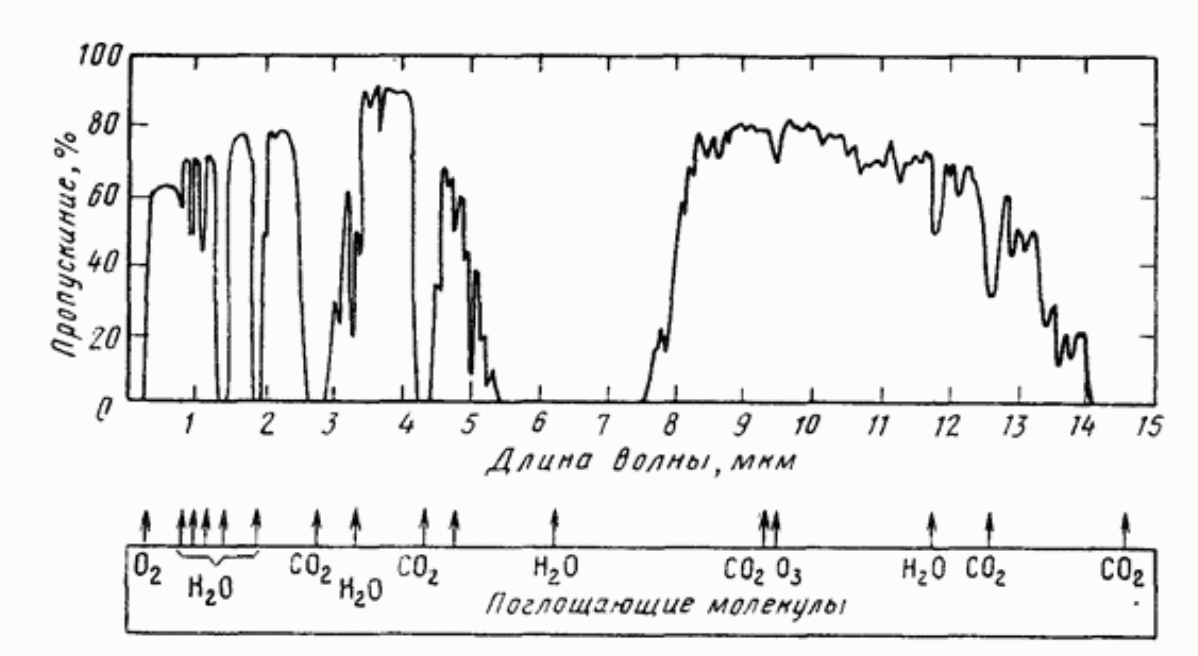
\includegraphics[width=0.7\linewidth]{2_atmosphere}
	\caption{Прозрачность земной атмосферы}
	\label{fig:2_atmosphere}
\end{figure}

\subsubsection{Гамма-астрономия в космосе}

Некоторая часть этого диапазона не доступна для наблюдений с Земли. Это самое жёсткое излучение. Гамма-диапазон – первый диапазон, освоенный астрономами в космосе. Первый астрономический спутник (Explorer 11) имел очень простые детекторы гамма-излучения.

Комптоновская гамма обсерватория: 4 прибора под разные участи этого диапазона. 

Сейчас на орбите находится обсерватория Fermi. 

Точность определения координат в этом диапазоне не очень велика.

Гамма телескопы  не совсем являются телескопами, так как мы не умеем фокусировать лучи (они или проходят сквозь, или слишком легко поглощаются при взаимодействии с веществом, а вот отражаются плохо…). Из-за этого по принципу устройства установки больше похожи на детекторы частиц (см. рисунок \ref{fig:2_fermi_lat}). По траекториям электронов и позитронов удаётся определять направление прилетающих  гамма квантов. Таким образом, направление на источник определяется по вторичным частицам. Энергия гамма квантов измеряется также косвенно по энергии позитронно-электронной пары.

\begin{figure}[H]
	\centering
	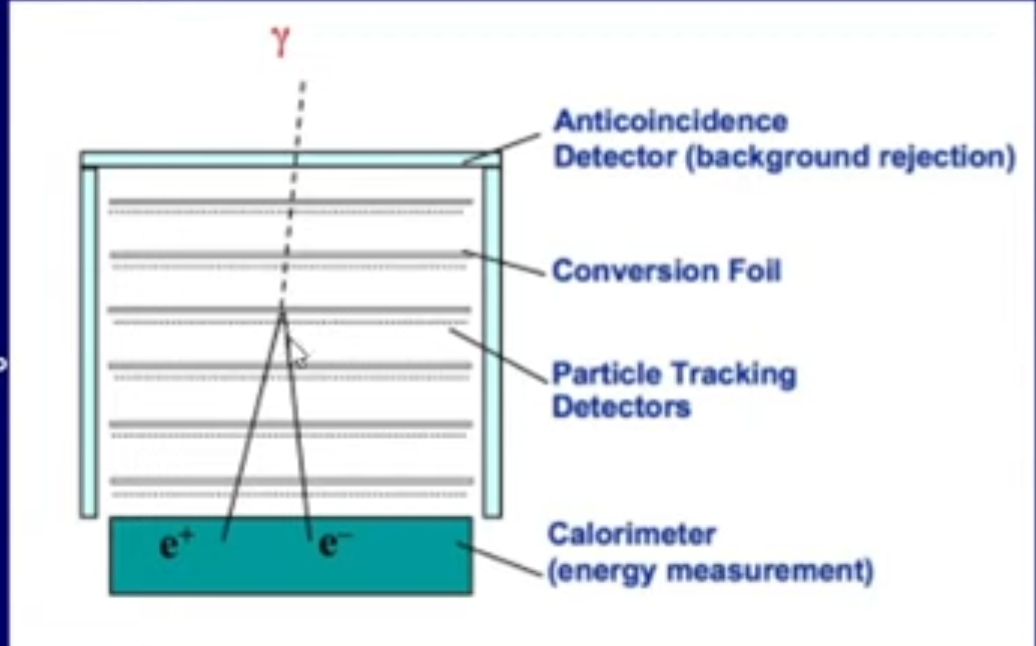
\includegraphics[width=0.7\linewidth]{2_fermi_lat}
	\caption{Ферми LAT}
	\label{fig:2_fermi_lat}
\end{figure}

\subsubsection{Рентгеновская астрономия}

\begin{itemize}
	\item Первые рентгеновские телескопы тоже были детекторами частиц. Сначала измерения проводились ракетами, летевшими по баллистической траектории (то есть время наблюдения очень небольшое). 
	
	\item Первый спутник UHURU (1970) - началась настоящая рентгеновская астрономия. Спутник RXTE, на котором стояли детекторы, которые фиксируют время прихода фотонов. Так как рентгеновских пульсаров очень не много в одном направлении наблюдения, то по периоду прихода фотонов можно определить, сигнал от какого источника получен. (\ref{fig:2_rentgen}) Как происходит регистрация? Есть камера, заполненная газом. Есть анод. Пролетает ионизирующая частица (в данном случае это квант рентгеновского излучения).  Летящая частица выбивает электроны, которые начинают двигаться к аноду. Но поданное напряжение ускоряет электроны, которые начинают выбивать другие электроны…Таким образом, результирующий сигнал усиливается, после чего мы измеряем ток, его легче регистрировать.
	
	\begin{figure}[H]
		\centering
		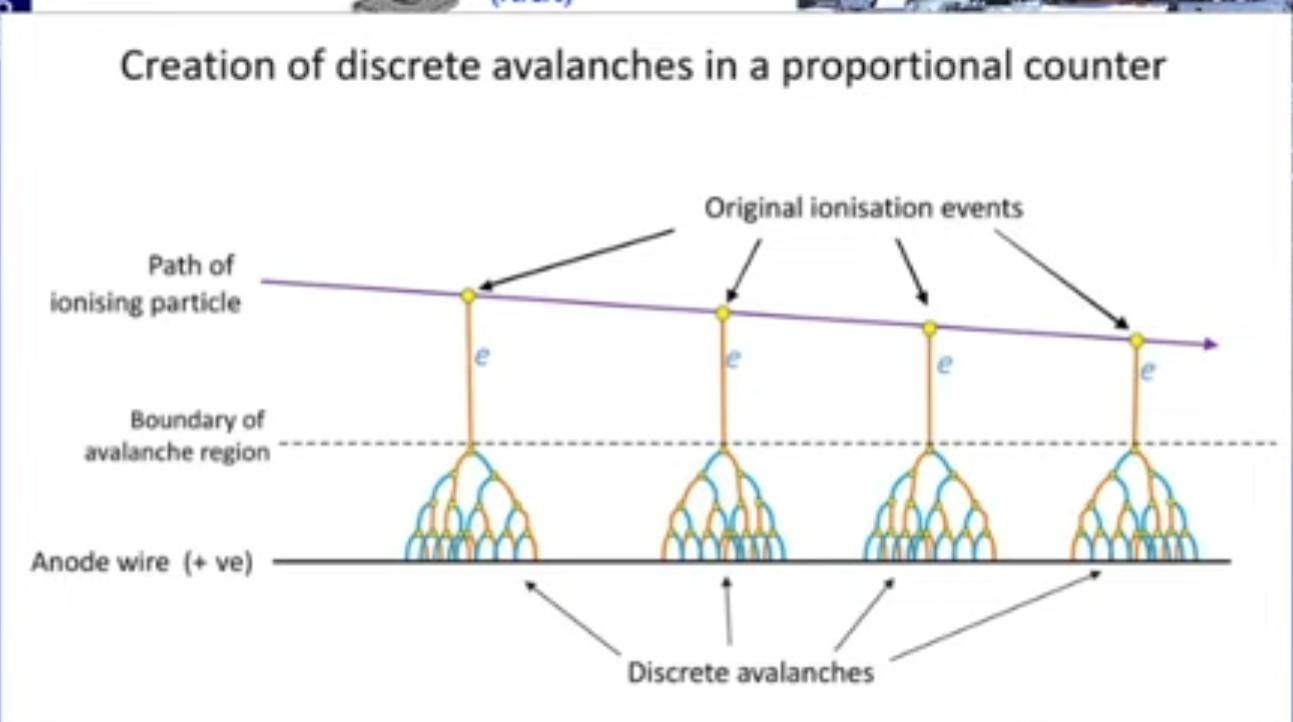
\includegraphics[width=0.7\linewidth]{2_rentgen}
		\caption{К методу работы рентгеновской астрономии}
		\label{fig:2_rentgen}
	\end{figure}
	
	\item Кодирующие маски. Отражений и преломлений всё ещё нет, но мы делаем шаг вперёд: улучшаем пространственное разрешение.  Теперь лучше понимаем, откуда прилетела частица. Реализовано на спутнике Integral. Кодирующая маска: сложная затемняющая картина (см. рисунок \ref{fig:2_code_mask}). Если мы будем смотреть на тени от источников, то тени будут достаточно причудливыми, поэтому будет легко  определять, где находятся источники. Улучшено угловое разрешение.
	
	\begin{figure}[H]
		\centering
		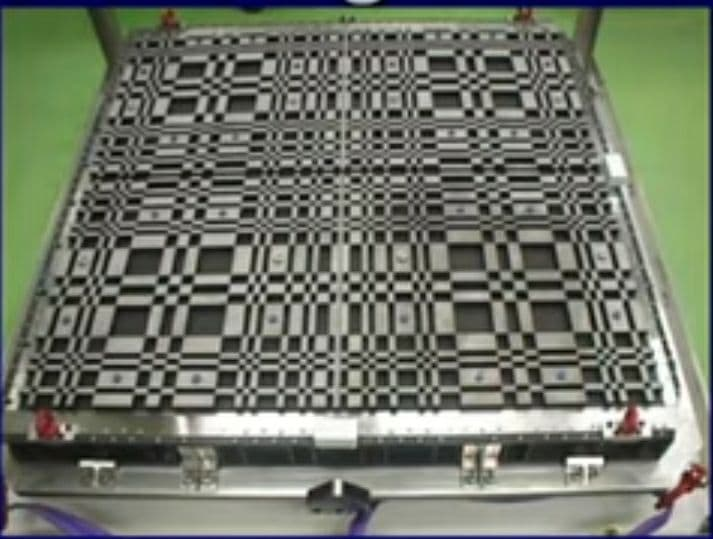
\includegraphics[width=0.7\linewidth]{2_code_mask}
		\caption{Кодирующая маска}
		\label{fig:2_code_mask}
	\end{figure}
	
	\item Современная рентгеновская астрономия. Появилась фокусирующая оптика. В 1979 году был запущен первый такой прибор. Сейчас на орбите два таких инструмента (Chandra и XMM-Newton). Как работает фокусировка? Зеркала косого падения. Рентгеновские кванты отражаются, но плохо. (Аналогия: можно бросить в воду кирпич, и он утонет, то есть не отразится. Можно бросить камень под очень маленьким углом к поверхности, и он будет многократно отражаться). Так и здесь: создаётся вложенная система зеркал, от каждого из которых отражение происходит под малым углом (см. рисунок \ref{fig:2_reflect}). Запускать такие телескопы сложно, так как система требует соосности зеркал с хорошей точностью.
	
	\begin{figure}[H]
		\centering
		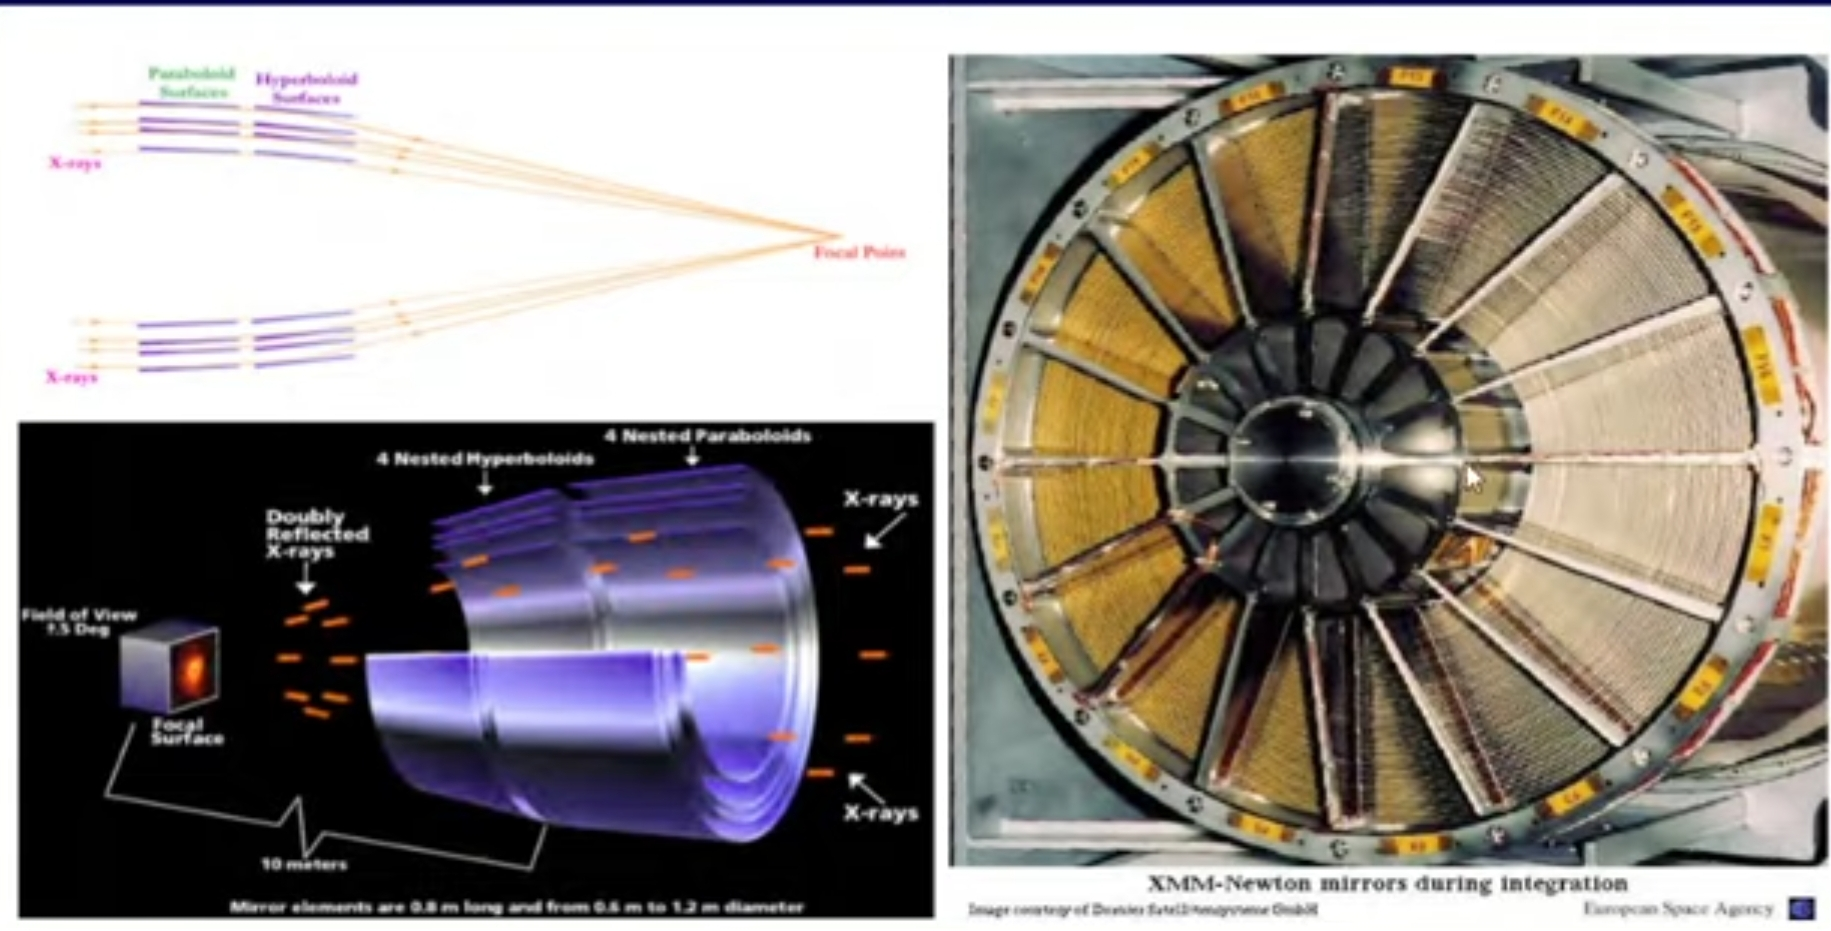
\includegraphics[width=0.7\linewidth]{2_reflect}
		\caption{Вложенная система зеркал}
		\label{fig:2_reflect}
	\end{figure}
	
	\item Идём в более короткие волны, т.е. угол падения должен быть ещё меньше, из-за чего система становится ещё длиннее, а это сложно. Решение: система  NuSTAR. Спутник состоит из двух частей. Отдельно летает оптика, и на расстоянии в несколько десятков метров от неё летает блок приёмной аппаратуры. Но это требует фантастической синхронизации. NuSTAR – раскладывающийся спутник (см. рисунок \ref{fig:2_NuSTAR}).
	
	\begin{figure}[H]
		\centering
		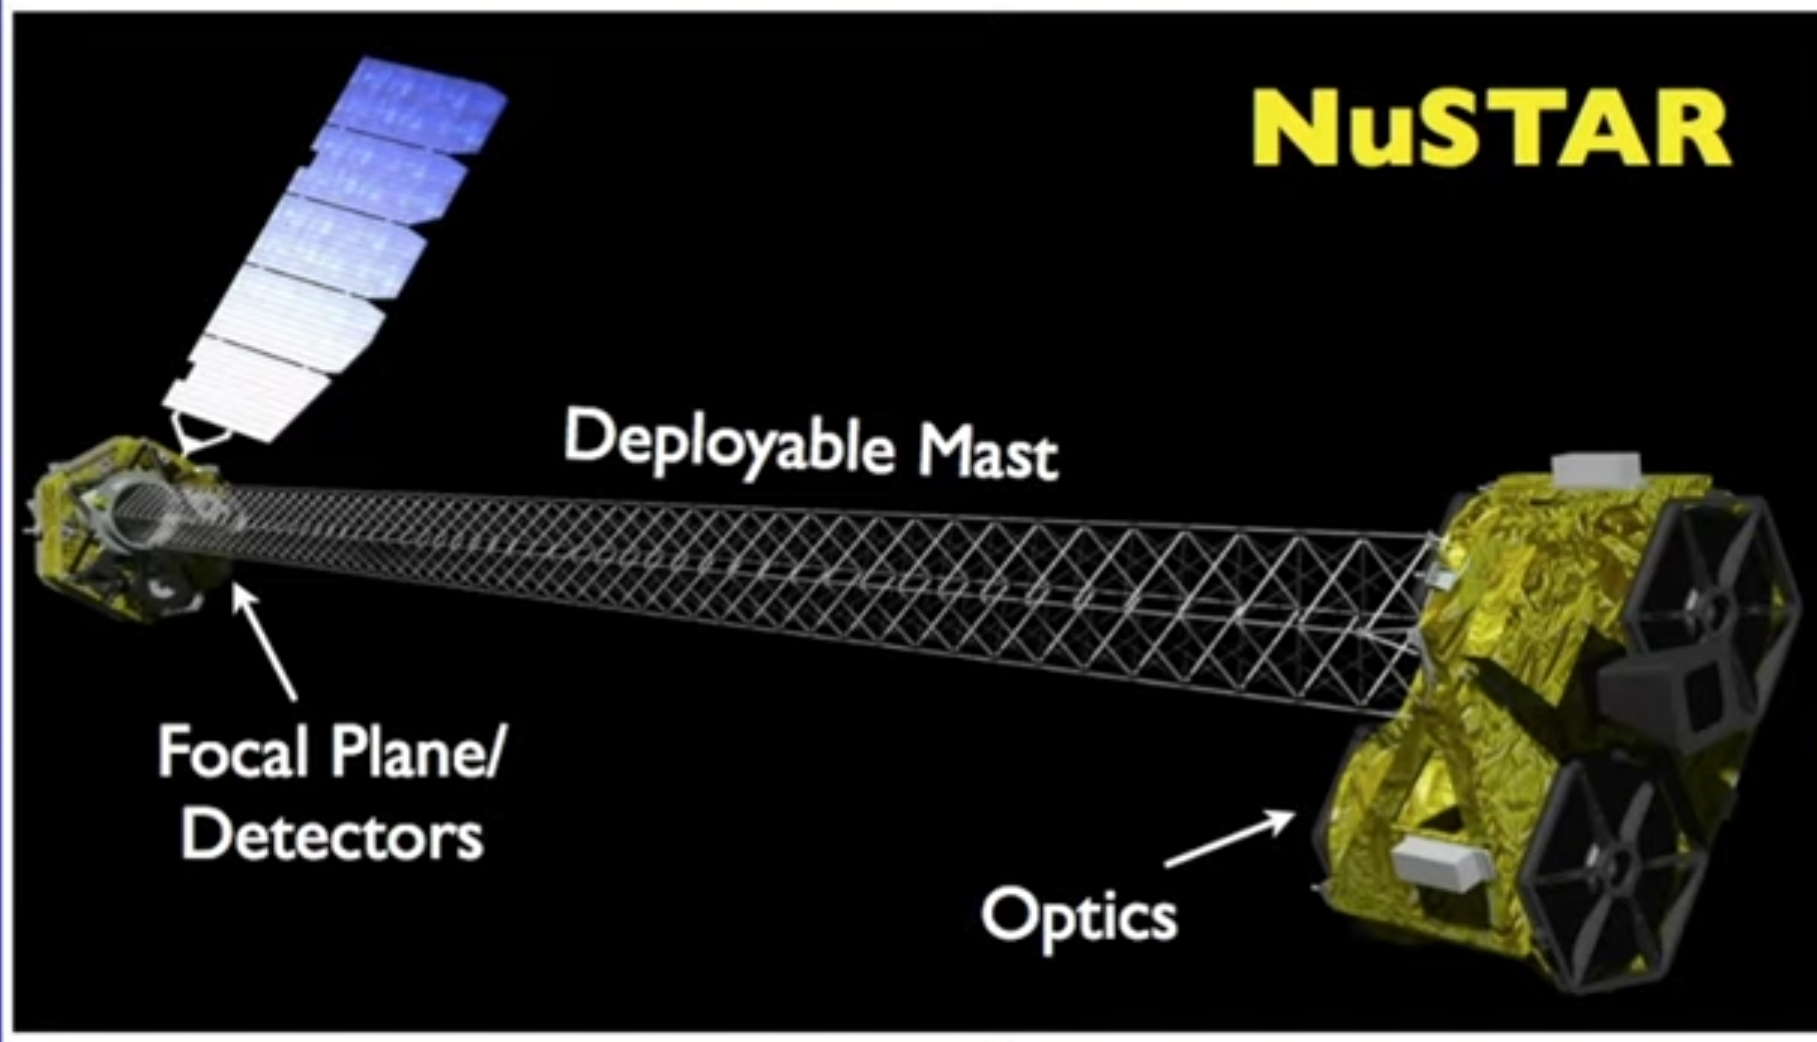
\includegraphics[width=0.7\linewidth]{2_NuSTAR}
		\caption{Спутник NuSTAR}
		\label{fig:2_NuSTAR}
	\end{figure}
\end{itemize}

\subsubsection{Инфракрасная астрономия}

Многие астрофизические процессы лучше наблюдать в ИК диапазоне, например, рождение звёзд и планет. Пример телескопа – «Спитцер».

С зеркалами тут всё проще, нам подходят привычные зеркала (почти как в оптическом диапазоне). При этом качество зеркало должно соответствовать длине волны, т.е. не требуется безумное качество поверхности. Однако есть проблема: всё вокруг излучает в этом диапазоне, даже люди! Чтобы решить эту проблему нужно охладить почти весь спутник жидким гелием, кроме того, нужно закрыть систему от Солнца специальным экраном. Но экран будет нагреваться и излучать…Эту проблему тоже надо решать. \textbf{Срок жизни спутника ограничен запасами жидкого гелия}. Но после исчерпания запасов жидкого гелия можно использовать телескопы в качестве неплохих в оптическом диапазоне.

Из интересных результатов в этом диапазоне: телескоп «Спитцер» смог восстановить карту распределения температуры по видимой поверхности планеты.

\subsubsection{Астрономия в оптическом и прилегающих диапазонах}

Телескоп имени Хаббла. Его диаметр всего 2.4 метра, однако он получил много важных результатов, так как ему не мешает атмосфера + длинные экспозиции. Он может строить изображения и получать спектры в видимом, ИК и УФ диапазонах. Способен наблюдать объекты до 31 звёздной величины.

Приборы Хаббла: некоторое время к нему можно было летать, поэтому несколько раз привозили современную аппаратуру. 

\medspace

\textbf{Астрометрические наблюдения}. Она тоже используют преимущества наблюдений из  космоса:  Gaia. Открытие экзопланет. Тут тоже мешает атмосфера.

\textbf{Большие установки}. Интерферометр на гравитационных волнах. Космический проект eLISA. 

\textbf{Космические лучи}. Изучение редких частиц высоких энергий. Находясь снаружи, мы можем наблюдать сразу за ~ половиной атмосферы Земли.

\textbf{Обзоры}. Можно «отсмотреть» всё небо одним прибором, а не «склеивать кусочки». С поверхности планеты так сделать нельзя. Например, нужно смотреть за реликтовым излучением именно на всём небе. Спутник Plank следил за реликтовым излучением.

Кроме того, может понадобиться постоянный мониторинг всего неба. Например, следим за потенциально опасными астероидами.




	
	\newpage
	
	
\section{Основные свойства Солнечной системы. Законы Кеплера}

Характерные размеры, числа, основные структуры Солнечной системы(СС). Вывод законов Кеплера.

\subsection{Структура СС. Характерные размеры}

Вокруг Солнца вращается целый комплекс объектов. Основная масса СС приходится на Солнце - его масса ~1.99$\cdot 10^{33}$ г., что составляет 99.86\% от массы СС.

Можно поделить СС на 5 основных групп(\textit{расположены в порядке удаления от Солнца}):

\begin{itemize}
	\item Планеты земной группы
	\item Пояс астероидов
	\item Планеты-гиганты
	\item Пояс Койпера
	\item (Рассеянный диск, о котором Попов совершенно не пишет в презентации)
	\item Облако Оорта
\end{itemize}

\subsubsection{Состав групп. Масштабы}

Деление на группы произведено по расстоянию и по типу объектов, входящих в состав группы. Из неочевидного, объекты пояса астероидов состоят в основном из горных пород и металлов; Здесь расположена одна из карликовых планет - Церера.

Объекты пояса Койпера же состоят в основном из летучих веществ(льдов) - метана, аммиака и воды, таким образом являясь возможным источником короткопериодических комет(например, комета Галлея с периодом 75-76 лет). Здесь расположены 4 оставшиеся карликовые планеты: Плутон, Эрида, Макемаке и Хаумеа.

Дальше идет Рассеянный диск, который содержит в себе такие же объекты, как и пояс Койпера, пересекаясь с последним, но простирается гораздо дальше от Солнца, и гораздо выше и ниже плоскости эклиптики.

Облако Оорта - это сферическая область СС, служащая источником долгопериодических планет, внешняя граница которой определяет гравитационную границу СС - на расстоянии около 2 св. лет.

Удобно для описания выражать расстояния до Солнца через \textbf{астрономическую единицу(a.u. или au)} - по определению, это(в приближении круговой орбиты) примерное расстояние от Солнца до Земли:

\begin{equation}
1 \text{ au} = 149 597 870 700 \text{ м.} \approx 150 \text{ млн. км.}
\label{eq:3_au}
\end{equation}

Тогда планеты земной группы - Меркурий, Венера, Земля, Марс - имеют орбиты ~0.3-0.47 au, ~0.71 au, ~1 au, ~1.38-1.67 au соответственно(интервалы - от наименьшего расстоянию(в перигелии) до Солнца, до наибольшего(в афелии)).

(Главный) пояс астероидов лежит в пределах ~2.06-3.27 au.

Планеты-гиганты - Юпитер, Сатурн, Уран, Нептун - имеют орбиты ~4.95-5.45 au, ~9-10.1 au, ~18.4-20.1, ~29.8-30.4 соответственно.

Пояс Койпера располагается на ~35-50 au от Солнца, Рассеянный диск на ~45-100 au(поэтому Эриду иногда причисляют именно к этому диску, потому что хоть и перигелий лежит в Поясе Койпера, большая полуось орбиты равна ~67.7 au).

Внешняя граница облака Оорта, по разным оценкам, составляет от 50000 до 200000 au.

\subsubsection{Размеры объектов}

Удобно для описания размеров планет и спутников использовать средний радиус Земли:

\begin{equation}
R_{\oplus} \approx 6371 \text{ км.}
\label{eq:3_r_earth}
\end{equation}

Для остального пользуемся старыми-добрыми км.

Основные элементы групп:

\begin{itemize}
	\item Планеты(о них следующий билет)
	\item Спутники - размеры от нескольких километров, до крупнейшего спутника Юпитера, имеющего радиус 0.413 земных.
	\item Планеты-карлики - объекты округлой формы, диаметром 400-2500 км.
	\item Астероиды - объекты неправильной формы, диаметром 1-1000 км.
	\item Кометы - объекты радиусом 1 - 10 км.
\end{itemize}

\subsection{Законы Кеплера}

Кеплер вывел эти 3 закона, вручную проанализировав огромное количество наблюдений. Их формулировка:


\begin{enumerate}
	\item Орбиты планет эллиптические, Солнце находится в одном из фокусов.
	\item Планета всегда заметает радиус-вектором одинаковую площадь за одинаковое время.
	\item Квадраты периодов(время, за которое планета проходит орбиту) относятся как кубы больших полуосей данных орбит.
\end{enumerate}

\begin{figure}[H]
	\centering
	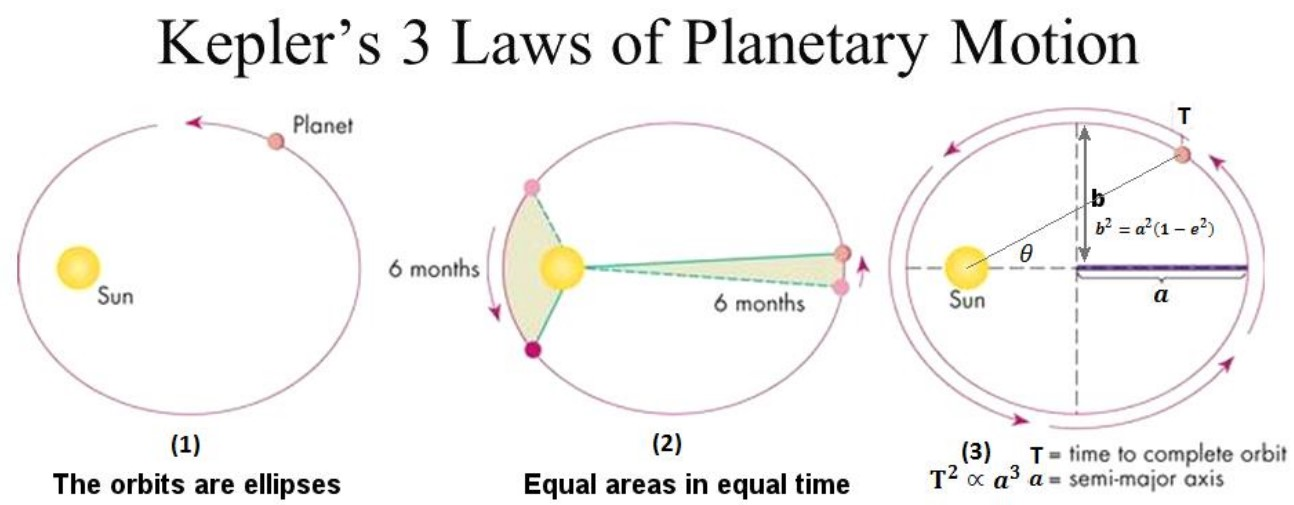
\includegraphics[width=0.7\linewidth]{3_kepler_laws}
	\caption{Графическое определение законов Кеплера}
	\label{fig:3_kepler_laws}
\end{figure}

\subsubsection{Подробнее о каждом законе}

Почему эллипсы? Ответ следует из закона сохранения энергии. Если еще и вспомнить, что сохраняется орбитальный момент L, то вывод упрощается:

\begin{figure}[H]
	\begin{subfigure}
		\centering
		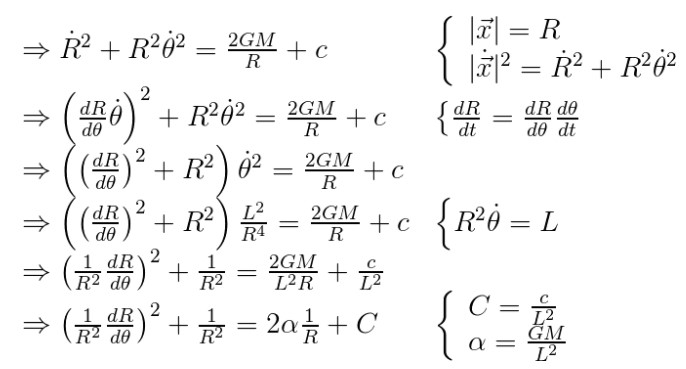
\includegraphics[width=0.7\linewidth]{3_ellipse_first}
	\end{subfigure}
	
	\begin{subfigure}
		\centering
		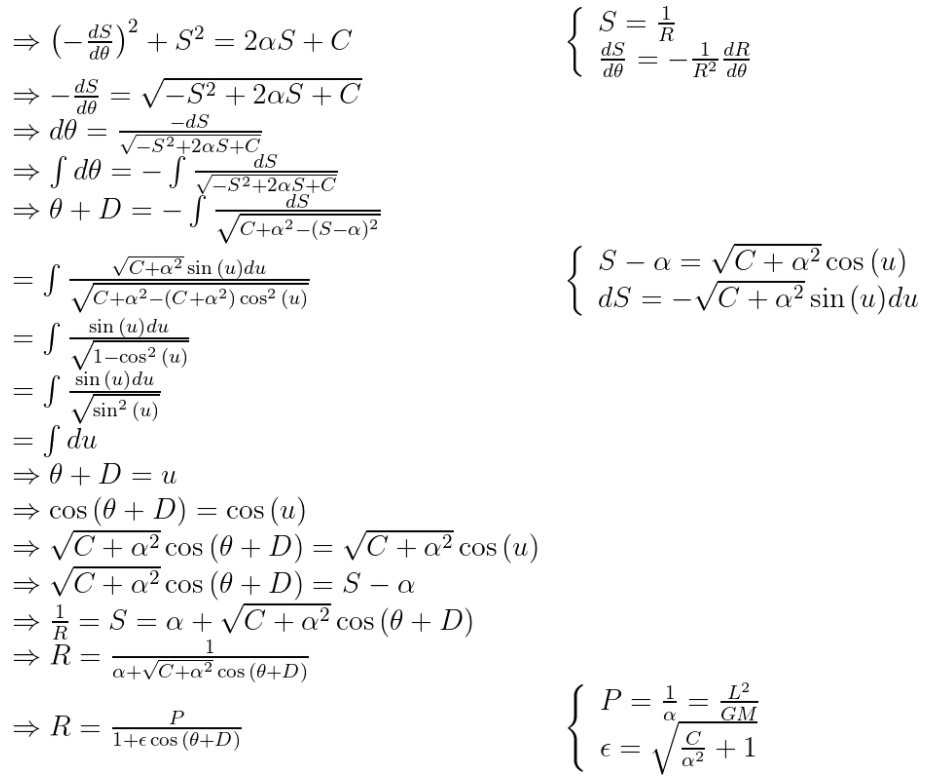
\includegraphics[width=0.7\linewidth]{3_ellipse_second}
	\end{subfigure}
	
	\caption{Связь радиуса и угла для эллиптической орбиты}
	\label{fig:3_ellipse}
\end{figure}

\textbf{Размер} большой полуоси зависит от полной энергии E, \textbf{форма(эксцентриситет)} - от орбитального момента L.

Второй закон - следствие сохранения орбитального момента:

\begin{eqnarray}
L = M_{pl} \cdot [\vec{r} \times \vec{V}] = const, \implies [\vec{r} \times \vec{V}] = const 
\label{eq:3_orb_moment}
\\
\text{Заметаемая площадь } \vec{dS} = [\vec{r} \times \vec{V}] dt, \implies \frac{\vec{dS}}{dt} = const
\label{eq:3_kepler_area}
\end{eqnarray}

Физическое следствие из этого - в ближайшей точке орбиты скорость тела наибольшая.

Третий закон можно вывести из второго закона Ньютона для притяжения тела к звезде, но является следствием закона сохранения энергии. Решая задачу двух тел и переходя к приведенной массе(M - масса звезды, m - масса планеты):

\begin{eqnarray}
\mu = \frac{Mm}{M + m}
\label{eq:3_reduced_mass}
\\
\frac{ \mu v^2 }{2 a} = \frac{GMm}{a^2}, v = \frac{2 \pi a}{P}, \text{считаем что $a_{st} \ll a_{pl} = a$}
\label{eq:3_newton}
\\
\implies P^2 = \frac{4 \pi^2}{G(M + m)} a^3 \text{ - уточнённая формулировка Третьего закона Кеплера}
\label{eq:3_kepler_third}
\end{eqnarray}

В приближении, что масса планеты много меньше массы звезды, можно пренебречь m в знаменателе и получится универсальная для звезды величина, связывающая период и большую полуось для орбит тел с маленькой массой, тем самым формулируя первоначальный(неточный) 3 закон Кеплера: "Квадраты периодов планет относятся как кубы больших полуосей".


	
	\newpage
	
	\section{Типы планет. Формирование планетных систем.}
\subsection{Классификация по составу}
\begin{wrapfigure}{r}{0.5\textwidth}
  \begin{center}
    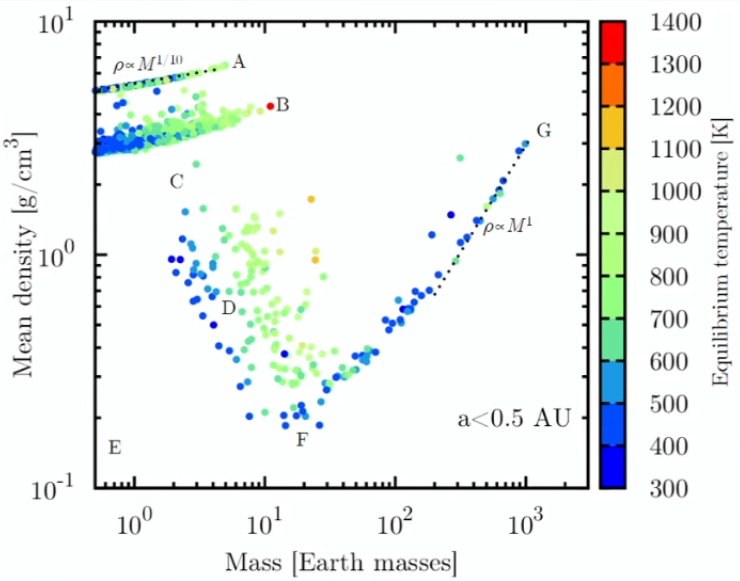
\includegraphics[width=0.48\textwidth]{Pictures/4_types.png}
  \end{center}
  \caption{График зависимости плотности планеты от ее массы: результаты моделирования. Цвет характеризует температуру планеты.}
  \label{fig:4_types}
\end{wrapfigure}
Основная классификация качественно представлена на графике \ref{fig:4_types}: 

A -- Твердые каменные. Плотность растет с увеличением массы, но очень медленно.

B -- Твердые ледяные. Плотность тоже растет медленно.

C -- Испаряющиеся.

D -- Маломассивные планеты с большими ядрами, тем не менее, обладающие толстой атмосферой, состоящая из легких элементов (водород и/или гелий). Такой состав атмосферы является причиной низкой средней плотности, при расчете которого учитывается \textit{видимый} радиус планеты.

E -- Запрещенная зона.

F -- Переход к планетам- гигантам.

G -- Планеты - гиганты. Газовые, следовательно, более сжимаемые объекты $\implies$ плотность растет быстро с ростом массы. 

\subsection{Основные типы планет}

\begin{wrapfigure}{l}{0.65\textwidth}
  \begin{center}
    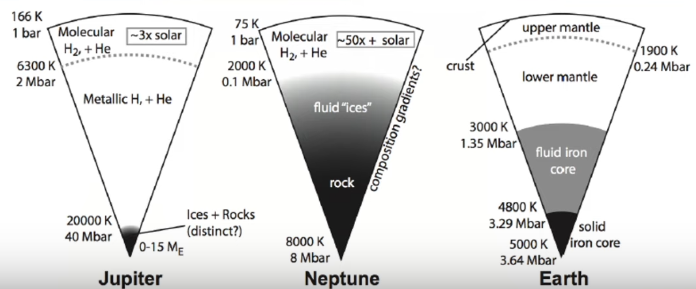
\includegraphics[width=0.63\textwidth]{Pictures/4_solar_types.png}
  \end{center}
  \caption{Типы планет}
  \label{fig:4_solar_types}
\end{wrapfigure}

Определяются \textit{основной} компонентой состава (рис.\ref{fig:4_solar_types}):

\paragraph{Газовые гиганты}: \textbf{H/He} (почти звездный состав). Планеты-гиганты, масса от 0.19 до 13 масс Юпитера. \textbf{Быстро вращаются.} Из-за колоссального давления в недрах планеты водород переходит в металлическую фазу (становится вырожденным). Радиус планет близок к радиусу \textbf{Юпитера}, или примерно в 10-11 раз превышает радиус Земли. Исключение составляют т.н. "горячие юпитеры" - планеты-гиганты, расположенные близко к своей звезде и имеющие эффективную температуру выше $1000\,\text{K}$. Сильно нагретая светом близкой звезды, их атмосфера расширяется, увеличивая видимый радиус планеты до 1-1.4 радиуса Юпитера. Средняя плотность гигантов меняется от 0.28 г/куб.см (самые разреженные горячие юпитеры) до 12 г/куб.см (самые массивные планеты-гиганты в 10-12 масс Юпитера). Скорее всего, все планеты-гиганты имеют сильное магнитное поле, усиливающееся с ростом массы планеты.

В Солнечной системе планеты-гиганты - Юпитер и Сатурн. 


\paragraph{Ледяные гиганты}: \textbf{H/He+лед+ядро. Нептуны}, масса от 7 до 60 масс Земли. Состоят большей частью из льдов (водяного, аммиачного, метанового, сероводородного) и скальных пород, составляющих примерно четверть полной массы планеты. Доля водорода и гелия в составе планеты не превышает 15-20$\%$. Давление в недрах недостаточно для перехода водорода в металлическую фазу. Радиус близок к 4 радиусам Земли. Средняя плотность составляет 1.3-2.2 г/куб.см. Магнитное поле сильно отличается от дипольного (например, планета может иметь два северных и два южных полюса).

В Солнечной системе нептуны - Уран и Нептун. 

\paragraph{Твердые планеты} \textbf{Si, Mg, Fe, C, O}. Железно-каменные планеты, планеты \textbf{земного типа}, масса меньше 7 масс Земли. Состоят в основном из силикатов и железа. Средняя плотность 3.5-6 г/куб.см. Радиус меньше 2 радиусов Земли.

В Солнечной системе планеты земного типа - Меркурий, Венера, Земля и Марс. 

\subsection{Формирование планетных систем}

\begin{wrapfigure}{r}{0.48\textwidth}
  \begin{center}
    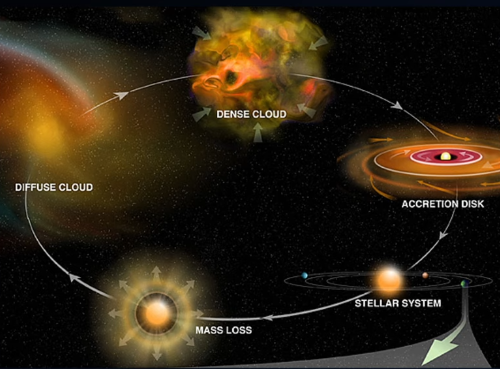
\includegraphics[width=0.5\textwidth]{Pictures/4_spiral.png}
  \end{center}
  \caption{Галактический спиралеворот: Формирование и распад планетной системы}
  \label{fig:4_spiral}
\end{wrapfigure}Существует много способов формирования планет. Основным путем образования планет считается путь снизу вверх (от мелких объектов к планетам).

Вокруг звезды, возникает протопланетный диск из смеси газа (которого много) и пыли (ее мало). Состав и свойства диска определяются межзвездной средой. В результате слияний, пылевые частицы начинают расти, вырастают в более крупные объекты. Если вокруг много газа, то эти объекты начинают его притягивать. Большие планеты растут из-за аккреции газа, а маленькие планеты растут слабо только за счет поглощения твердых объектов. Вблизи солнца образуются маленькие каменные планеты, потому что тяжелых элементов мало, а дальше, где газа много, образуются газовые гиганты. Большие планеты всегда обязаны быть газовыми, потому что только водорода и гелия много. Вблизи звезды начинает плавиться пыль ($\ge 1300\,\text{K}$), но при удалении от звезды температура падает (по закону Стефана-Больцмана). 

\paragraph{Снеговая линия} Многие газы могут замерзать, образовывая ледяные пылинки. Снеговая линия -- критическое расстояние от звезды, на котором температура достаточно низкая для этого процесса, соответственно, внутри снеговой линии не могут существовать и расти ледяные тела. Для Солнца она находится примерно на расстоянии 3 а.е.

Достаточно тяжелые ледяные объекты, начинают корректировать газ и возникает ледяной гигант. 
\newpage
\subsubsection{Миграция планет}

\begin{wrapfigure}[17]{l}{0.3\textwidth}
  \begin{center}
    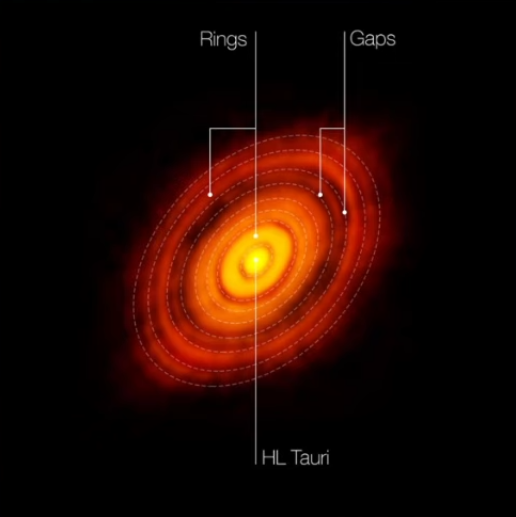
\includegraphics[width=0.28\textwidth]{Pictures/4_disk_gaps.png}
  \end{center}
  \caption{Протопланетный диск HL Тельца}
  \label{fig:4_disk}
\end{wrapfigure}Планета не сохраняется на одном радиусе, мигрируя преимущественно внутрь системы из-за взаимодействия с веществом диска и ''расталкивая'' его. 
При взаимодействии с частицей с меньшим радиусом орбиты, планета притягивает и тормозит ее, уменьшая ее полную энергию. Следовательно, частица переходит на \textit{более низкую} орбиту. Аналогично планета отталкивает частицы, находящиеся снаружи своей орбиты.

Однако не все планеты создают такую щель, как на \mbox{рисунке \ref{fig:4_disk}}. Если планета не достигла критической массы, взаимодействие будет слабым и вещество будет ''протекать''. Если же планета открывает щель, ее миграция замедляется.

Однако, создав щель, планета не перестает расти. Таким образом, планета служит мостом для передачи вещества и углового момента, ''протекающих'' через нее.(рис. \ref{fig:4_brige})
Миграция оказывает влияние на вид системы и может значительно поменять ее вид. 
\begin{wrapfigure}[23]{r}{0.4\linewidth}
  \begin{center}
    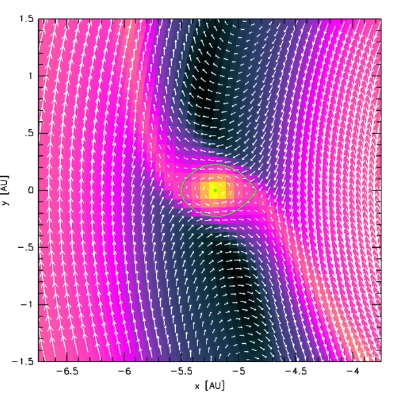
\includegraphics[width=\linewidth]{Pictures/4_brige.png}
  \end{center}
  \caption{''Мост''}
  \label{fig:4_brige}
\end{wrapfigure}
Причина, по которой планетные системы выглядят сжатыми (вся ''жизнь'' происходит в одном месте, близко к звезде по сравнению с размерами системы), заключается во взаимодействии планет при миграции. Миграция массивных внешних планет сдвигает более мелкие, внутренние планеты к центру системы.

С течением времени планета становится все массивнее, и влияние на диск -- заметнее.

\paragraph{Фанфакты}

\begin{itemize}

    \item \textbf{Эффект Лидова-Козаи} В системе трёх тел у орбиты может меняться одновременно и эксцентиситет, и наклон. Этим объясняется движение планет в системе в противоположные стороны (изначально все планеты находятся в одной плоскости и движутся в одном направлении).  
    \item \textbf{Приливы} Если планета находится блико к звезде, она будет возбуждать прилив, который будет приводить к торможению планеты, сл, переход на более низку орбиту, и, в конечном счете, разрушение/поглощение звездой. Событие редкое. Еще планета может испариться/перетечь в звезду.

    \item \textbf{Цикличность} Процесс образования новых звезд планетных систем идет непрерывно, как и выброс вещества в межзвездную среду (\mbox{рис. \ref{fig:4_spiral}}). На каждом последующем цикле появляется больше тяжелых элементов (первые звезды не могли иметь каменные планеты).
    
    \item \textbf{Фрагментация диска} Крупные планеты могут образовываться на больших расстояниях (за снеговой линией, 10 а.е и больше) от звезды как результат неустойчивости диска: гравитационно связанные объекты сжимяется и мигрирует, преврящаясь в планету в бурые карлики. Ситуация редкая ($\sim$ 1$\%$ планет)
    
\end{itemize}

	
	\newpage
	
	\section{Методы регистрации экзопланет, преимущества и недостатки разных методов.}
\subsection{Изменение лучевой скорости звезды (вращение вокруг центра масс системы звезда-планета)
}
Смотрим на спектр звезды вокруг которой вращается экзопланета, за счет эффекта Доплера спектр будет вмещаться в синюю/красную сторону, когда движется к нам/от нас 
Благодаря этому измеряем орбитальный период звезды, орбитальный период планеты, соответсвенно, такой же. Зная массу звезды находим массу экзопланеты

Ситуация осложняется, когда планет много. 
\subsection{Транзитный метод}
Визуально, конечно, не можем увидеть. Наблюдаются флуктуации блеска звезды. Блеск падает на очень маленькую величину (1000-ые доли), также мешает земная атмосфера, тем не менее изменения все равно регистрируются, особенно для крупных экзопланет, сейчас транзиты наблюдают со спутников.

Вероятность транзита составляет порядка 1\% (ДЗ 3).

\paragraph{Задача}
Рассчитайте вероятность транзита, если радиус звезды равен $R_{\star} = 0.5 R_{\Sun}$ ($R_{\Sun}$ -- радиус Солнца),
а большая полуось (круговой) орбиты $a = 0.1$ а.е. Радиус планеты $R_{\circ} = 1.4R_{\Jupiter}$ ($R_{\Jupiter}$ -- радиус
Юпитера). 
Положение наблюдателя считать случайным с равновероятным распределением. Отдельно рассчитать вероятность полного транзита $\mathcal{P}_{whole}$ (весь диск планеты проецируется на диск звезды) и частичного $\mathcal{P}_{partial}$, а также суммарную вероятность $\mathcal{P}_{\Sigma}$.
\paragraph*{Решение:}
\begin{figure}[H]
    \centering
    \begin{tikzpicture}[scale=1.5,>=latex']
    \filldraw[blue!22!white] (4.8,2*0.1032795559) -- (4,0) -- (4.8,-2*0.1032795559) -- cycle;
    \filldraw[blue!22!white] (-1,1.290994449) -- (4,0) -- (-1,-1.290994449) -- cycle;
    \filldraw[fill=yellow!55!white] (0,0) circle (1);
    \filldraw[] (0,0) circle (0.02);
    \draw[<->] (-1,0) -- (0,0) node[above,pos=0.5]{$R_{\star}$};
    \filldraw[xshift=4.4cm,fill=black!55!white] (0,0) circle (0.1); 
    \draw[xshift=4.4cm] (-0.1,0.2) -- (-0.1,-1);
    \draw[xshift=4.4cm] (0.1,0.2) -- (0.1,-1);
    \draw[xshift=4.4cm,->] (-0.5,-0.9) -- (-0.1,-0.9);
    \draw[xshift=4.4cm,->] (0.5,-0.9) -- (0.1,-0.9);
    \node[] at (4.4,-1.2){$2R_{\circ}$};
    %\draw (0.25,0.9682458) -- (0,0);
    \draw[] (-1,1.290994449) -- (4.8,-2*0.1032795559);
    \draw[] (-1,-1.290994449) -- (4.8,2*0.1032795559);
    \draw[dashed] (-1,1.23056316956) -- (48.4/9,-0.0978857);
    \draw[dashed] (-1,-1.23056316956) -- (48.4/9,0.0978857);
    \draw (0,0) -- (0,1.5);
    \draw[xshift=4.4cm] (0,0) -- (0,1.5);
    \draw[<-] (0,1.3) -- (2.1,1.3);
    \draw[->] (2.3,1.3) -- (4.4,1.3);
    \node at (2.2,1.3) {$a$};
    %\draw[<-] (0,0) -- (2.1,0);
    %\draw[->] (2.3,0) -- (4.4,0);
    %\node at (2.2,0) {$a$};
    \filldraw[xshift=4.4cm] (0,0) circle (0.02);
    \end{tikzpicture}
    \caption{Рисунок к задаче 1. Планета (тёмно-серая) может проецироваться на звезду (жёлтая) полностью (голубая область), а может частично (выделена пунктиром).}
    \label{prmlm_1pic}
\end{figure}
Из рисунка~\ref{prmlm_1pic} легко получить соотношения для вероятностей и их значения, учитывая $R_{\Sun} \approx 10R_{\Jupiter} =\approx 0.47\cdot10^{-2} $ а.е.:
\begin{multline*}
    \mathcal{P}_{whole} = \frac{R_{\star} - R_{\circ}}{a} = \frac{0.5R_{\Sun} - 1.4R_\Jupiter}{a} \approx \frac{0.5R_{\Sun} - 0.14_{\Sun}}{a} =\\ = \frac{0.36R_{\Sun}}{a} \approx \frac{0.36\cdot 0.47\cdot 10^{-2}}{0.1} \approx \boxed{1.7\%} 
\end{multline*}
\begin{multline*}
    \mathcal{P}_{\Sigma} = \frac{R_{\star} + R_{\circ}}{a} = \frac{0.5R_{\Sun} + 1.4R_\Jupiter}{a} \approx \frac{0.5R_{\Sun} + 0.14_{\Sun}}{a} =\\ = \frac{0.64R_{\Sun}}{a} \approx \frac{0.64\cdot 0.47\cdot 10^{-2}}{0.1} \approx \boxed{3.0\%} 
\end{multline*}
\begin{equation*}
    \mathcal{P}_{partial} = \mathcal{P}_{\Sigma} - \mathcal{P}_{whole} = 3.0 - 1.7 = \boxed{1.3\%}
\end{equation*}
\subsection{Микролинзирование}
Если близко к лучу зрения между наблюдаемой звездой и наблюдателем попадает объект (может быть что угодно, планетах черная дыра и тд), то объект искажает пространство-время вокруг себя, работает как гравитационная линза. Блеск звезды будет возрастать по мере того как линза будет все ближе подлетать к лучу зрения, а потом симметрично убывать.

 Если линза состоит из нескольких объектов, в нашем случае массивная звезда и экзопланета, то в изменении регистрируемого блеска будет возникать небольшой пик от планеты.

Плюс метода в том что единичное наблюдение гарантирует результат, не нужно долго копить данные. Линзирования также работает на очень удалённых объектах, что нехарактерно в других методах. 
\begin{figure}[H]
    \centering
    \includegraphics[scale=0.4]{mcrl.png}
    \caption{Микролинзирование}
    \label{fig:mcrl}
\end{figure}
\subsection{Тайминг}
Если мы наблюдаем систему в которой происходят какие-то периодические события, то наличие внешних объектов буду приводить к изменению преиода. Например, для пульсаров будет возникать эффект доплера из-за вращения вокруг центра масс системы пульсар-экзопланета.

\subsection{Астрометрическое детектирование}
Самый старый и неточный способ. Мы не видим планету, но можем измерить, что меняется положение звезды, т.к. она вращается вокруг центра масс системы. Метод требует очень высокой точности измерений 
\subsection{Выделение вклада планеты в общее излучение системы}
Например, в случае транзитной планеты (если она является достаточно мощным
 источником собственного или отраженного излучения) мы можем увидеть не только падение блеска системы при транзите, но и рост блеска в те моменты, когда одновременно виден и весь диск звезды, и диск планеты. Таким способом удалось изучить свойства нескольких планет, например в системе Кеплер-70. Вклад планеты можно выделить и изучая спектры. Линии, излучаемые планетой, во-первых, будут соответствовать другим скоростям и смещаться (из-за эффекта Доплера) относительно звездных линий. А во- вторых, по свойствам линий можно понять, что они связаны с относительно холодным веществом. Этот метод также успешно используется. В нескольких десятках случаев удалось получить непосредственные изображения молодых экзопланет.
\subsection{Непосредственное наблюдение}
Эти методом можно обнаружить только очень крупные, нагретые, удалённые от звезды планеты в силу того, что планеты являются очень слабыми источниками. Не смотря на ограниченные возможности этого метода таким способом обнаружено несколько десятков планет.

	
	\newpage
	
	\input{TeX_files/6.tex}
	
	\newpage
	
	\section{Солнечная активность и её изменения со временем}

Внешняя структура Солнца от внутренних к внешним:

\begin{itemize}
	\item Фотосфера – видимый диск. На определенном радиусе на определенной длине полны Солнце перестает быть прозрачным (оптическая толщина примерно равна 1).
	
	\item Хромосфера – цветной ореол вокруг Солнцы, его «внутренняя атмосфера».
	
	\item Корона --- часть внешней атмосферы Солнца, очень разреженная и протяжённая часть.
\end{itemize}

Основной механизм охлаждения фотосферы --- это излучение, а основным механизмом ее нагрева служат поднимающиеся из недр Солнца мелкомасштабные конвективные потоки (более крупные конвективные ячейки, ответственные за появление крупномасштабной хромосферной сетки, находятся глубже). Выход конвективных потоков наблюдается как мелкомасштабная ячеистая структура фотосферы, образуемая непрерывно возникающими и исчезающими областями повышенной яркости — гранулами — с довольно резкими границами. Характерный размер гранул \~ 1500 км., а время их существования --- 5-10 минут. Скорости конвективных потоков не превышают нескольких км/с. Газ поднимается, остывает и опускается вниз между ячейками за новой порцией энергии. В отдельных областях фотосферы, как правило, вблизи солнечных пятен, наблюдаются протяженные области повышенной яркости, образуемые цепочками многочисленных более «горячих» гранул. Это \textbf{факелы}, или \textbf{факельные поля} — долгоживущие образования (могут существовать месяцами), связанные с более интенсивным конвекционным переносом тепла из нижележащих слоев Солнца. Напряженность магнитного поля в факелах составляет несколько сотен Гауссов — недостаточно для того чтобы затормозить конвекцию. Температура газа в факелах на несколько сотен К выше окружающей поверхности. 

Самыми заметными деталями фотосферы являются солнечные пятна. \textbf{Солнечные пятна} – области активности. Пятна тёмные, так как там ниже температура (примерно на 1500К). Подвод тепла к ним осуществляется снизу, но в области пятен подвод тепла подавляется сильным магнитным полем. 

Пятна связаны с Солнечной активностью. Пятен больше, когда Солнце активнее. Нет, Солнце не светит слабее в это время, ведь за энерговыделение отвечают термоядерные реакции внутри (а пятна обусловлены процессами во внешних слоях звезды)

\subsection{Про подавление конвекции под пятнами}

Каждое пятно — это место выхода в атмосферу из недр Солнц а трубки силовых линий магнитного поля. Поскольку эти линии замкнутые, они образуют широкую петлю над фотосферой. Обычно пятна образуются парами в местах входа и выхода силовых линий поля петли (биполярная структура). Если средняя индукция поля в фотосфере Солнца порядка 1 Гаусса, то в пятнах она составляет от нескольких сотен до нескольких тысяч Гауссов. Плотность энергии поля при этом достаточно велика, чтобы в силу вмороженности поля в газ затормозить конвекцию, препятствуя движению газа по замкнутым линиям тока. Резкое уменьшение притока энергии из недр Солнца и является причиной локального падения температуры и образования пятна. Энергия, не достигшая фотосферы в области пятен, частично выходит на поверхность благодаря усиленной конвекции в факелах. Группы пятен вместе с окружающими их факелами называют активными областями на Солнце. Силовые линии магнитных полей, связанных с активными областями, могут уходить высоко в верхние слои солнечной атмосферы, где они подчиняют себе движение сильно разреженного ионизованного газа. Поэтому над активной областью структура магнитного поля, как и поле скоростей газа, и его плотность, оказываются крайне неоднородными.

И солнечные вспышки, и корональные выбросы — это результат преобразования энергии магнитного поля в другие формы энергии, вызванного развитием плазменных неустойчивостей в магнитном поле со сложной конфигурацией силовых линий. Частота появления таких событий меняется как из месяца в месяц, так и из года в год — в такт изменению общей активности Солнца. 

\textbf{Солнечные вспышки.} Это ещё одно проявление активности Солнца. В результате пересоединения линий магнитного поля выделяется энергия. Полное энерговыделение не очень большое, но энергия выделяется быстро.

Если вспышка сопровождается выбросом плазмы (около $10^{15}$ г) – \textbf{корональные выбросы}. Выброшенная плазма может взаимодействовать с атмосферой земли, долетая до неё за 1-4 дня.

Солнечные вспышки наблюдать трудно. Их обнаруживают из-за увеличения потока УФ и радиоизлучения. Однако были и визуальные наблюдения астрономами-любителями, кроме того, есть данные по геомагнитному шторму. Так, в длинных проводниках могут наводится большие токи, увеличивается активность полярных сияний.

Солнечные вспышки — лишь наиболее яркое проявление активных процессов на Солнце. Под активностью Солнца понимают целый комплекс явлений в различных слоях его атмосферы, обусловленных выходом магнитных полей в активных областях. Над активными областями атмосфера Солнце по всей ее толщине имеет более высокую плотность и температуру, и поэтому обладает более высокой яркостью в коротковолновом диапазоне. Горячий газ образует многочисленные петли самых различных размеров, отражающие структуру силовых линий магнитного поля. Эти петли отчетливо наблюдаются в мягких рентгеновских лучах. Подъем активности Солнца проявляется в более частом образовании как активных областей фотосферы, так и очень горячих очагов в короне над центрами активности, более частом образовании солнечных вспышек и корональных выбросов.

\subsection{Цикл солнечной активности (Швабе, 1843)} 

Этот цикл связан с изменением глобального магнитного поля Солнца. Глобальное магнитное поле Солнца \~ 1 Гаусс. За 11 лет меняется полярность поля, оно переворачивается. (То есть совсем честный полный цикл 22 года). 

Активность Солнца подвержена изменениям с периодом, лежащим в пределах 8–13 (в среднем 11) лет. Есть указания на существование колебаний активности с более короткими и с более длинными периодами, но они выражены не столь явно, как 11-летний цикл. Рост очередного цикла активности начался в конце 2009 г. В годы минимума на Солнце может в течение долгого времени не наблюдаться никаких пятен или вспышек, а в годы максимума иногда одновременно существуют десятки пятен, образующие отдельные группы. Далекое УФ и рентгеновское излучение Солнца как звезды также подвержено резким колебаниям, отражающим уровень солнечной активности. Меняется с циклом активности и общий вид короны, отражающий конфигурацию крупномасштабного магнитного поля. В минимуме активности структура поля более простая, близкая к дипольной, и корона вытянута вдоль экватора. Вблизи максимума она становится более сферически симметричной. Корональные лучи, наблюдаемые в любой фазе цикла, дают начало «спокойному» солнечному ветру, интенсивность которого также подвержена изменениям и связана с уровнем активности Солнца.

Таким образом, активность Солнца претерпевает некоторую эволюцию, которая плохо описана. Наблюдалось несколько минимумов активности, самый известный из которых – маундеровский (см. рисунок \ref{fig:7_sunspot}).

\begin{figure}[H]
	\centering
	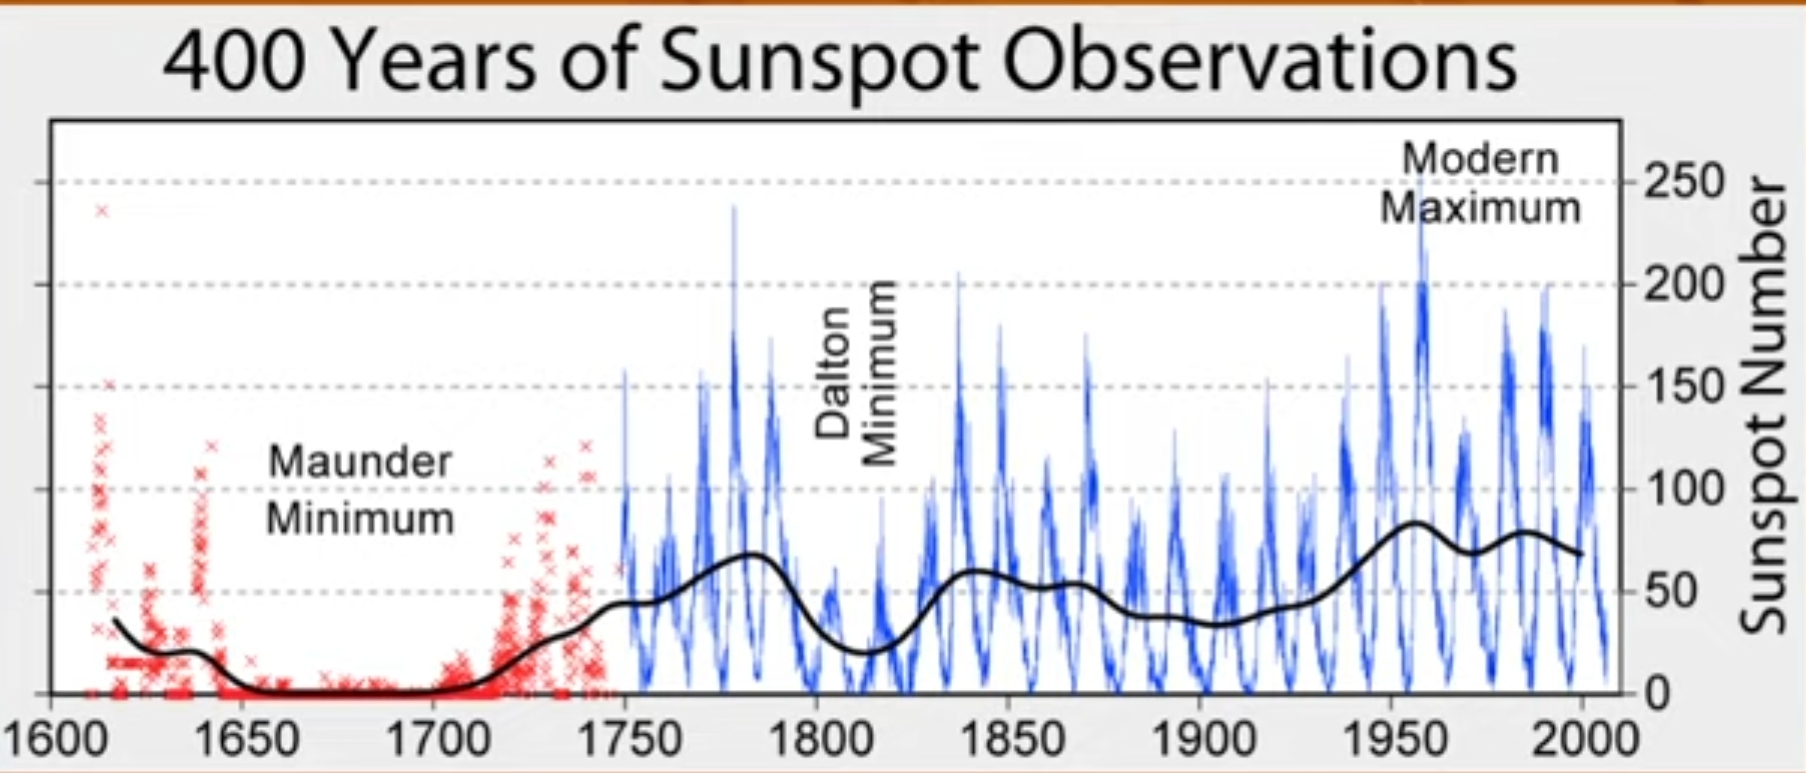
\includegraphics[width=0.7\linewidth]{7_sunspot}
	\caption{Солнечная активность от года}
	\label{fig:7_sunspot}
\end{figure} 

Мощные солнечные вспышки и корональные выбросы влияют на физические условия в космическом пространстве, в магнитосфере и ионосфере Земли, ее радиационных поясах. Высокая радиация может вывести из строя электронную космическую аппаратуру или представлять опасность для космонавтов. Наибольшее влияние солнечной активности испытывают внешние, ионизованные слои земной атмосферы. Но опосредованно активность Солнца сказывается и на поверхности Земли, на многих явлениях живой и неживой природы — от роста нестабильности атмосферной циркуляции до увеличения частоты сердечно-сосудистых кризов. Отдельные звенья сложных цепочек, обуславливающих связь земных явлений с активностью Солнца, пока плохо изучены. Уровень активности Солнца отслеживается и прогнозируется в ряде стран специальными службами Солнца.

\subsection{Реконструкция солнечной активности на большом масштабе времени}

Учёные пытаются восстановить солнечную активность на временах порядка тысяч лет. Это делается с помощью анализа содержания космогенных изотопов. Эти изотопы образуются в верхней атмосфере Земли под действием галактических космических лучей. То есть это частицы высоких энергий, которые прилетают в нашу систему откуда-то. Внутри гелиосферы доминирует солнечный ветер, то есть поток от Солнца мешает космическим лучам проникать внутрь Солнечной системы. Поэтому, когда активность Солнца выше, поток галактических космических лучей на уровне верхней атмосферы Земли меньше. Это приводит к тому, что образуется меньше, например, бериллия-10 и углерода-14. Поэтому, анализируя относительную долю этих изотопов в различных образцах, если мы умеем датировать эти образцы, можно делать выводы об активности Солнца. Например, можно анализировать ледяные керны и годичные кольца деревьев и говорить что-то об активности Солнца в далёком прошлом. Удаётся получить точность в несколько десятилетий.

\textbf{Глобальная эволюция Солнца}. Эта эволюция происходит на масштабе миллиарда лет, она никак не связана с описанными выше ~ 50ти летними минимумами и максимумами.

	
	\newpage
	
	
\section{ Синтез элементов во вселенной.}

До образования звезд обычное вещество в основном существовало в виде водорода(самый распространенный элемент) и гелия. Т.о., большая часть химических элементов, с которыми мы сталкиваемся в жизни, возникли в звездах в течение их жизни или на последних стадиях жизни массивных звезд - взрывах сверхновых.

\subsection{Явления во вселенной}

Чтобы показать, откуда появились те или иные элементы, привожу картинку, на которой каждому элементу сопоставлен(ы) способ(ы) его образования.

\begin{figure}[H]
	\centering
	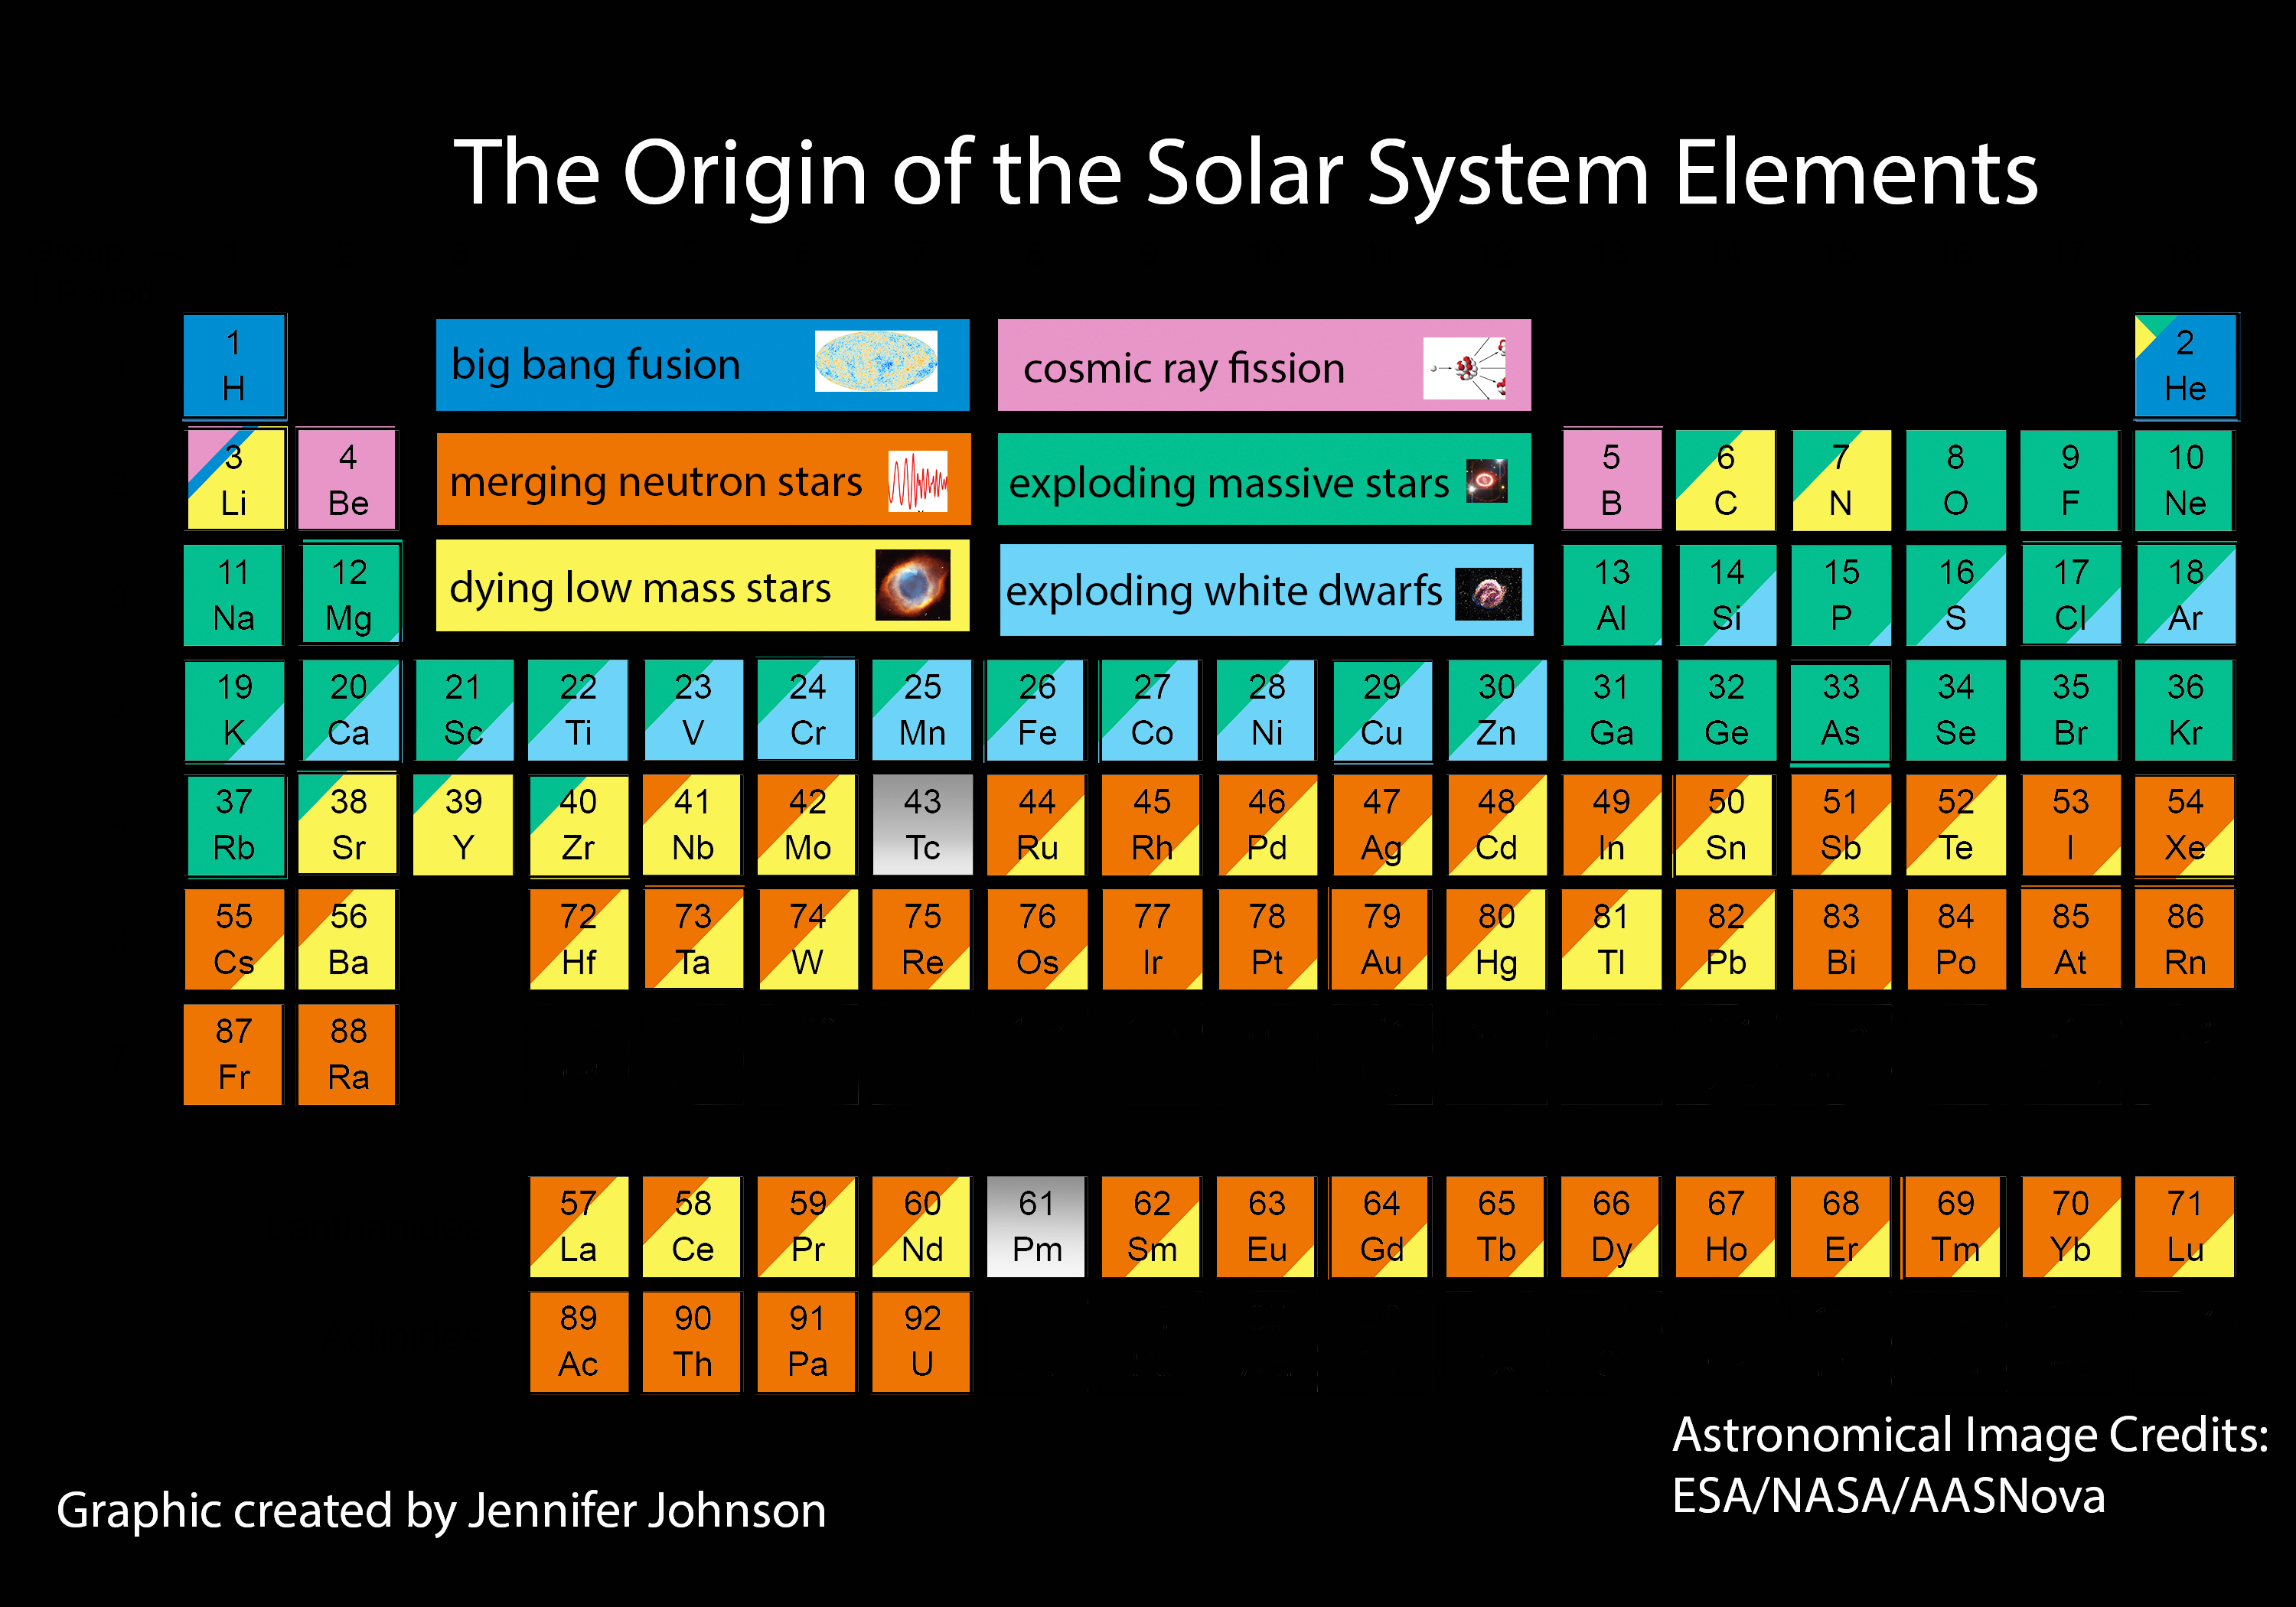
\includegraphics[width=0.7\linewidth]{8_periodic}
	\caption{Своеобразная таблица Менделеева}
	\label{fig:8_periodic}
\end{figure}

Разберем по цветам(пойду по строчкам):

\colorbox{Blue}{Big bang fusion} - слияние Большого взрыва; это те элементы, которые были до существования первых звёзд.

\colorbox{CarnationPink}{Cosmic ray fission} - это \href{https://en.wikipedia.org/wiki/Cosmic_ray_spallation}{"Реакция скалывания"}. Они происходят уже вне звёзд - сейчас существуют различные тяжелые элементы во вселенной. Космические лучи(частицы с высокой энергией), налетая на более тяжелые элементы, "модифицируют" их создавая как один из продуктов Бериллий/Бор/Литий. В звездах Бериллий и Бор не синтезируются - термоядерные реакции проскакивают с Гелия сразу до Углерода.

\colorbox{BurntOrange}{Merging neutron stars} - процесс слияния нейтронных звезд. Крайне важный и крайне редкий процесс(в нашей галактике - раз в ~30000 лет(по словам Попова)), который является источником самых тяжелых элементов.

\colorbox{SeaGreen}{Exploding massive stars} - \textbf{гравитационный коллапс} ядра массивной звезды, при котором часть оболочки сбрасывается, тем самым выбрасывая новые элементы. Происходят в нашей галактике раз в ~30 лет.

\colorbox{Yellow}{Dying low mass stars} - умирающие маломассивные звезды. Элементы синтезируются в оболочках этих красных гигантов. Взрыва не происходит - недостаточно массы, но звезда превращается в белый карлик, сбрасывая с себя оболочку которую мы называем планетарной туманностью.

\colorbox{Cyan}{Exploding white dwarfs} - термоядерный взрыв белого карлика. В основном синтезируются элементы группы Железа.

\subsection{Основные термоядерные реакции}

Теперь поговорим о термоядерных реакциях, происходящих в этих процессах. Нам \textbf{не важно} то, что происходит в ядрах звёзд! Потому что синтезирующиеся там элементы в этом ядре и остаются, например, создавая в конце жизни звезды углеродно-кислородный белый карлик(судьба нашего Солнца). Выделяют два основных процесса:

\begin{enumerate}
	\item S-процесс - Slow, медленный
	\item R-процесс - Rapid, быстрый
\end{enumerate}

S-процесс идёт в оболочках звезд-гигантов. Есть два процесса, создающих свободные нейтроны в звезде(рис. \ref{fig:8_neutrons}). Эти нейтроны легко проникают в ядра(у них нет заряда), увеличивая массу ядра, а затем, подвергаясь бета-распаду, синтезируют элементы с все большим зарядом. Так получаются элементы массой до ~100 и от ~138 до ~208. Процесс может идти миллионы лет.

\begin{figure}[H]
	\begin{subfigure}
		\centering
		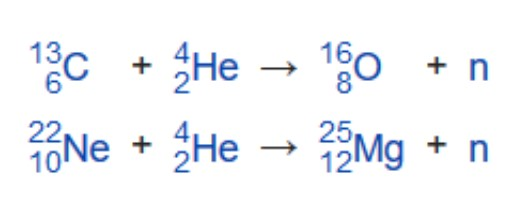
\includegraphics[width=0.7\linewidth]{8_neutrons}
		\caption{Реакции с выделением свободных электронов}
		\label{fig:8_neutrons}
	\end{subfigure}
	
	\begin{subfigure}
		\centering
		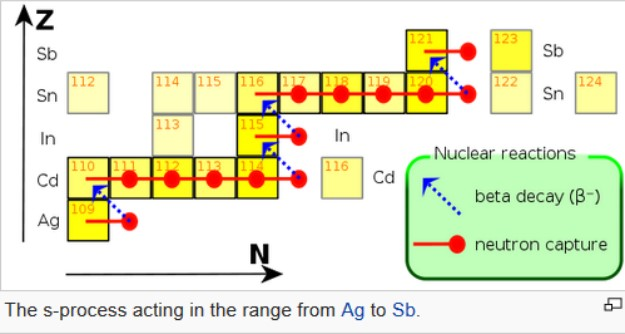
\includegraphics[width=0.7\linewidth]{8_slow}
		\caption{Пример S-процесса}
		\label{fig:8_slow}
	\end{subfigure}

	\label{fig:8_s_process}
\end{figure}

R-процесс идёт во вспышках сверхновых и при слиянии нейтронных звёзд. Временной масштаб тут намного меньше S-процесса: речь идет о секундах. Происходит всё при высокой плотности нейтронов, в результате получаются насыщенные нейтронами ядра, заряд ядра как и в случае медленного процесса увеличивается засчет бета распада. В результате получаются элементы вплоть до Урана.

\begin{figure}[H]
	\centering
	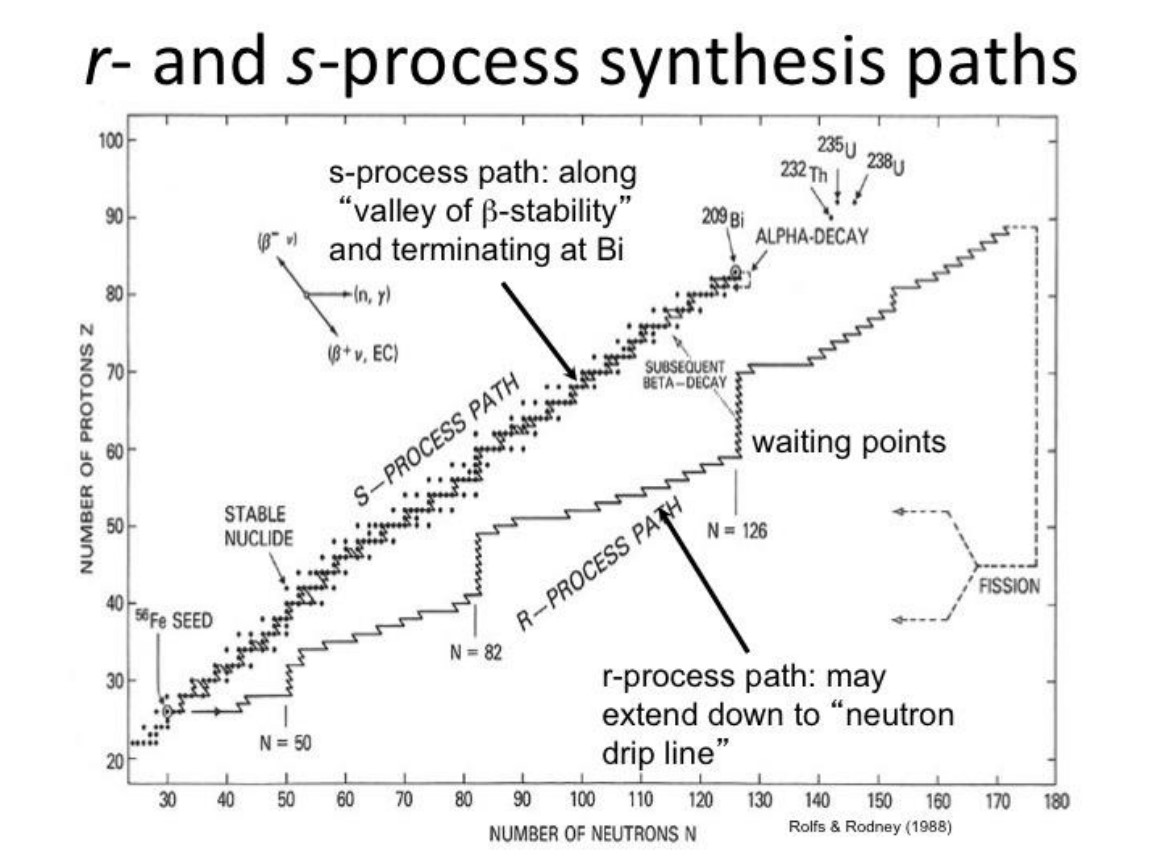
\includegraphics[width=0.7\linewidth]{8_comparison}
	\caption{Сравнение путей по которым могут идти s- и p- процессы}
	\label{fig:8_comparison}
\end{figure}

	
	\newpage
	
	\section{Эволюция звезд –- основные стадии.}

\subsection{Образование звезд}

Звёзды образуются из областей гравитационной неустойчивости в облаках межзвёздного газа. 

\paragraph{Масса Джинса}

Чтобы началось звездообразование, нужно, чтобы полная энергия была отрицательной, то есть, (по теореме вириала) если гравитационная энергия по модулю больше удвоенной кинетической.

Критическая масса, при которой \textit{может} начаться звездообразование называется массой Джинса.

\begin{equation*}
2 K + U = 0 \implies
 \begin{cases}
   K = N \frac{3}{2} k T\\
   U = - \frac{3}{5}\frac{GM^2}{R}
 \end{cases} \implies
 N k T = \frac{M}{m} k T = \frac{GM^2}{5R} = \frac{GM^2}{5}\left(\frac{4\pi\rho}{3 M}\right)^{1/3}
\end{equation*}

\begin{equation}
   \boxed{ M_j = \left(\frac{5 k T}{Gm} \right)^{3/2} \left(\frac{3}{4\pi\rho} \right)^{1/2}}
   \label{eq:9_jeans}
\end{equation}

Из формулы \ref{eq:9_jeans} видно, что звезды формируются из более \textbf{плотных} и \textbf{холодных} областей -- именно они начнут коллапсировать. 

Изначально сжимется большой фрагмент облака ($> 10^3 M_{sun}$) (поэтому часто звезды образуются \textit{скоплениями}). По мере сжатия растет плотность, но не температура (облако прозрачно для собственного излучения, которое уносит энергию), джинсовская масса падает и объект разделяется на более мелкие, имеющие звездные/субзвёздные массы. Есть причины полагать, что таким образом могут формироваться не только звезды, но и бурые карлики, и может быть планеты.

\paragraph{Первые звезды}

Таким образом формировались первые звезды (100 млн лет после Большого взрыва), так как состояли только из легких элементов. Газу было трудно остывать, потому что излучение провоцируют колебательные уровни молекул(типа C-O, которые в ранней Вселенной еще не сформировались). Таким звездам было трудно достичь низких джинсовых масс, так как единственная существовавшая колебательная молекула для них H-H. Они были большие, жили мало (1-2 млн лет) и быстро взрывались как сверхновые, распространяя тяжелые элементы 

\paragraph{Теорема вириала для звезд}

Звезды являются очень стабильными объектами, так как отвод тепла заставляет звезду сжиматься, а значит нагреваться, и наоборот, нагрев влечет за собой расширения и псоледующее остывание. Можно сказать, что звезды обладают ''отрицательной теплоемкостью'' или ''обратной связью''.

\newpage

\subsection{Популяции звезд}

Выделяют три типа популяции (населения) звезд:
\begin{figure}
    \centering
    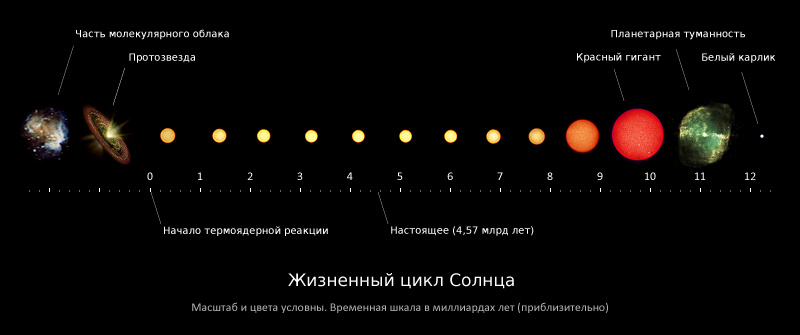
\includegraphics[width = 0.9\textwidth]{Pictures/9_Solar-evolution.png}
    \label{fig:9_solar}
\end{figure}

\begin{itemize}
    \item Популяция III -- самые первые звёзды.
    
    Состоят из водорода и гелия -- первичного газа Вселенной.
    \item Популяция II -- старые звёзды Галактики.
    
    \item Популяция I -- ''современные'' звёзды (до 10 млрд. лет назад).
    Особенность -- хим. состав (содержание тяжелых элементов).
    
\end{itemize}
\subsection{Эволюция звезд}

Классифицировать звезды удобно с помощью диаграммы \textbf{Герцшпрунга - Рассела}. 
\begin{wrapfigure}[18]{r}{0.63\linewidth}
  \centering
    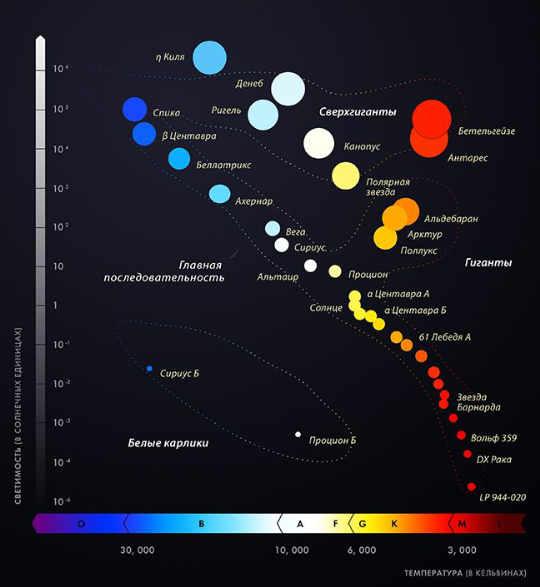
\includegraphics[width=0.65\linewidth]{Pictures/9_diag.png}
  \caption{Диаграмма Герцшпрунга-Рассела}
  \label{fig:9_diag}
\end{wrapfigure}Это зависимость светимости звезды от температуры (чем левее, тем горячее). В реальности не получалось точно измерять эти параметры,  поэтому по горизонтальной оси откладывали спектральные характеристики, а по вертикальной -- звездную величину для данного скопления. Оказалось, что подавляющее большинство звезд ложится на одну линию, которую назвали \textit{главная последовательность}. 90$\%$ жизни звезды проводят, находясь на главной последовательности, так как она соответствует стадии превращения водорода звезды в гелий.

\newpage

\begin{figure}[h]
\begin{minipage}[h]{0.49\linewidth}
\center{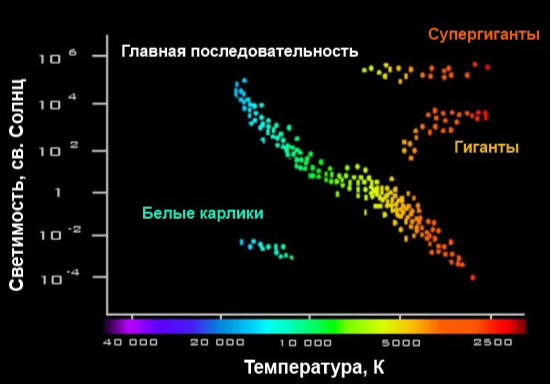
\includegraphics[width=0.9\linewidth]{Pictures/9_life.png} \\ а) Главная последовательность}
\end{minipage}
\hfill
\begin{minipage}[h]{0.49\linewidth}
\center{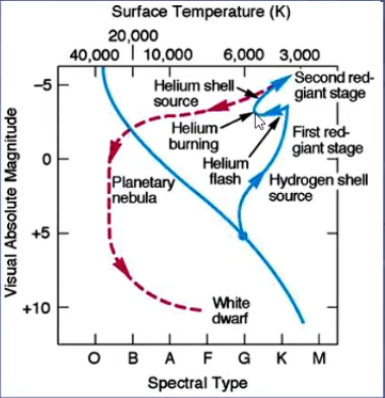
\includegraphics[width=0.6\linewidth]{Pictures/9_life2.png} \\ б) Эволюция Солнца}
\end{minipage}
\caption{Эволюция одиночной звезды.}
\label{fig:9_life}
\end{figure}

\begin{itemize}
    
    \item После того, как весь водород в ядре заканчивается, теряется источник энергии. Звезда остывает (теряет энергию), а значит, сжимается (становится более плотным), от этого нагревается. Этот процесс будет происходить, пока не появятся условия для начала термоядерного горения ядра. Не для всех звезд это возможно. 
    
    \item Из-за сжатия повышается температура и плотность на внешней границе ядра (вне ядра все еще есть водород). Если возникают условия для начала термоядерных реацкия \textit{вне} ядра, водород становится \textbf{слоевым источником} очень большой мощности. Резко растет светимость звезды, она расширяется и превращается в \textbf{красный гигант}.
    
    \item Ядро внутри сжимается. Если достигаются условия горения гелия в ядре, звезда уходит с ветки красных гигантов (рис. \ref{fig:9_life} (б) ), ее температура повышается при постоянной светимости.
    
    \item Гелий в ядре заканчивается (быстрее, чем водород, температуры выше). Образуется углеродно - кислородное ядро, наступает вторая стадия красного гиганта (\textbf{гигант - асимптотическая ветвь}).
    
    \item Ядро сжимается и пытается перейти на следующую стадию. У маломассивных звезд (типа Солнца) ядро начнет остывать, сбрасывать внешнюю оболочку, будет уменьшаться светимость и образуется \textbf{белый карлик}. В дальнейшем он будет остывать, переходя вправо по линии спектральных классов (горизонтальная ось рис. \ref{fig:9_life} (а) ).
    
    \item Если звезда достаточно массивная, в ядре начинается горение углерода и кислорода, звезда взрывается и превращается в нейтронную звезду или чёрную дыру.
    
\end{itemize}

\newpage

\subsection{Особенности треков для звезд разной массы}

\paragraph{Протозвезды} -- объекты высокой светимости (из-за того что она сжимается) и низкой температуры. Излучение преимущественно в инфракрасном диапазоне.

\paragraph{Массивные звезды} Для массивных здезд есть неопределенности, поэтому расчеты не согласуются между собой полностью, но общая черта заключается в значительно меньшем размере петли трека(рис. \ref{fig:9_life} (б) ), чем для звезд сравнимых по массе с Солнцем. 


    
\paragraph{Фанфакты} 

\begin{itemize}
    \item Чем меньше металличность звезды, тем раньше она образовалась.
    \item Возраст звезды на главное последовательности трудно определить.
    \item Основная характеристика звезды -- масса. Чем больше масса, тем больше звезда излучает и тем меньше живет.
    \item Время жизни звезд с массой меньше солнечной сравнимо с временем жизни галактики.
    \item \href{http://nuclphys.sinp.msu.ru/m_un/mun16.htm}{Полезная ссылочка}, а тут \href{https://habr.com/ru/post/366947/}{красивые картиночки}.
\end{itemize}

	
	\newpage
	
	\section{Белые карлики: основные свойства, образование, новые и сверхновые типа Ia}
\subsection{Общие сведения}
Белые карлики -- компактные объекты большой плотности, образующиеся в результате эволюции звёзд не привыкающих массы $\sim 10M_{\Sun}$. Когда звезда главной последовательности малой или средней массы заканчивает превращение водорода в гелий, она расширяется, становясь красным гигантом. Красный гигант поддерживается термоядерными реакциями превращения гелия в углерод и кислород. Если масса красного гиганта оказывается недостаточной для подъёма температуры ядра до уровня, необходимого для термоядерных реакций с участием полученного углерода, происходит его накопление в ядре звезды, вместе с кислородом. Звезда сбрасывает внешнюю оболочку, формируя планетарную туманность, а бывшее ядро звезды становится белым карликом, состоящим из углерода и кислорода.

Ближайший известный белый карлик — Сириус B, находящийся на расстоянии в 8,6 световых лет. В настоящее время белые карлики составляют, по разным оценкам, от 3 до 10\% звёздного населения нашей галактики (неопределённость оценки обусловлена трудностью наблюдения удалённых белых карликов из-за их малой светимости).

В зависимости от исходной массы звезды, термоядерные реакции также могут остановиться на гелии (для звёзд с очень малой массой, характерных для двойных звёздных систем) или на неоне (для звёзд массой от 8 до 10,5 солнечных), что приведёт к образованию белых карликов, состоящих соответственно из гелия или кислорода, неона и магния.

Образующийся объект имеет массу порядка солнечной, однако его диаметр может быть в $\sim 100$ раз меньше.  
\subsection{Предел Чандрасекара}
Как уже упоминалось, массы белых карликов составляют порядка солнечной, но размеры составляют лишь сотую (и даже меньше) часть солнечного радиуса, то есть плотность вещества в белых карликах чрезвычайно высока и составляет $\rho \sim 10^{5}-10^{9} \ \frac{\text{г}}{\text{см}^{3}} $. При таких плотностях электронные оболочки атомов разрушаются, и вещество представляет собой электронно-ядерную плазму, причём её электронная составляющая представляет собой вырожденный электронный газ. Давление $P$ такого газа подчиняется следующей зависимости:
\begin{equation*}
    P = K\rho^{\frac{5}{3}}
\end{equation*}
Вышеприведённое уравнение состояния действительно для холодного электронного газа, но температура даже в несколько миллионов градусов мала по сравнению с характерной ферми-энергией электронов (
$kT\ll E_{F}$). Вместе с тем, при росте плотности вещества из-за запрета Паули (два электрона не могут иметь одно квантовое состояние, то есть одинаковую энергию и спин), энергия и скорость электронов возрастают настолько, что начинают действовать эффекты теории относительности — вырожденный электронный газ становится релятивистским. Зависимость давления $P$ релятивистского вырожденного электронного газа от плотности уже другая:
\begin{equation*}
    P = K\rho^{\frac{4}{3}}
\end{equation*}
Средняя плотность белого карлика ($M$ -- его масса, $R$ -- радиус):
\begin{gather*}
    \rho \propto \frac{M}{R^{3}}\\
    P\propto \frac{M^{\frac{4}{3}}}{R^{4}}
\end{gather*}
Cила давления, противодействующая гравитации и равная перепаду давления по глубине:
\begin{equation*}
    \frac{P}{R}\propto \frac{M^{\frac{4}{3}}}{R^{5}}
\end{equation*}
Гравитационные силы, противодействующие давлению:
\begin{equation*}
    \frac{\rho G M}{R^{2}} \propto \frac{M^{2}}{R^{5}}
\end{equation*}
то есть, хотя перепад давления и гравитационные силы одинаково зависят от радиуса, но по-разному зависят от массы. Следствием такого соотношения зависимостей является существование некоторого значения массы звезды, при которой гравитационные силы уравновешиваются силами давления, а при увеличении массы белого карлика его радиус уменьшается. Другим следствием является то, что если масса больше некоторого предела (предел Чандрасекара), то звезда коллапсирует. Предел Чандрасекара -- $1.2M_{\Sun}$. 
\begin{figure}[H]
    \centering
    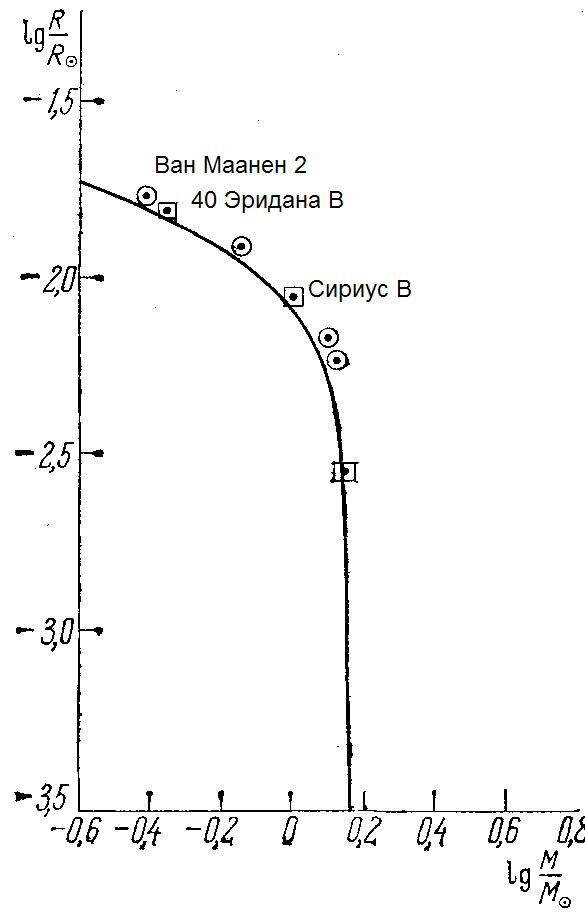
\includegraphics[scale=0.5]{10_white_dwarf.png}
    \caption{Кривая радиус -- масса (нормированная и логарифмированная) для белых карликов.}
    \label{fig:wd}
\end{figure}
\subsection{Сверхновые типа Ia}
\subsubsection{Аккреционный механизм}
Если белый карлик является одной из звёзд двойной системы, то он может начать аккрецировать массу со второй звезды, тем самым наращивая свою массу. В некоторых случаях накопив массу близкую к пределу Чандрасекара карлик может взорваться сверхновой.

При взрыве температура в ядре достигает миллиарда градусов, а значительная часть вещества белого карлика, состоявшего в основном из кислорода и углерода, за несколько секунд превращается в более тяжёлые элементы и выбрасывается в окружающее пространство со скоростями до 5 000 — 20 000 км/с, что составляет примерно 6 \% от скорости света. Выделенной энергии ($1—2\cdot10^{44}$ Дж) достаточно чтобы полностью разорвать звезду, то есть отдельные её составляющие части получают достаточно кинетической энергии, чтобы преодолеть гравитацию.

\subsubsection{Механизм слияния}
Существует и другой механизм запуска термоядерных реакций. Белый карлик может слиться с другим белым карликом (не менее 80\% всех сверхновых Ia типа по одним данным, менее 15 \% или даже как чрезвычайно редкое по другим) и на короткое время может превысить предел массы и начать коллапсировать, снова поднимая свою температуру до достаточной для ядерного синтеза. В течение нескольких секунд после начала ядерного синтеза со значительной частью вещества белого карлика происходит быстрая термоядерная реакция с выделением большого количества энергии ($1—2\cdot10^{44}$ Дж), вызывающая взрыв сверхновой звезды.

	
	\newpage
	
	
\parindent=1cm

\section{Сверхновые с коллапсом ядра и формирование нейтронных звезд. Ключевые параметры
нейтронных звезд.}

\subsection{Сверхновые с коллапсом ядра}
Одним из двух типов сверхновых будет сверхновая с коллапсом ядра. В этом случае энергия высвобождается за счет коллапса ядра массивной звезды. В зависимости от того, теряет ли звезда водородную оболочку, сверхновые делятся на два типа.

\begin{figure}[H]
\centering
\includegraphics[width=0.7\linewidth]{11_1.png}
\caption{B - сверхновая без водородных линий, C - сверхновая с остатками водородной оболочки}
\end{figure}

В случае сверхновой с коллапсом звезды -- начальный этап: ядро звезды размером десятки тысяч километров. Далее происходит сжатие ядра до нейтронной звезды с характерным размером около 10 км. Характерная энергия взрыва: $\frac{GM^2}{r} \sim 10^{53}$ эрг , M -  масса ядра (приблизительно равна массе Солнца), r - радиус нейтронной звезды. 

\begin{figure}[H]
\centering
\includegraphics[width=0.6\linewidth]{11_2.png}
\caption{Кривая блеска сверхновой}
\end{figure}


Максимум блеска достигается при движении ударной волны к поверхности звезды в результате взрыва. Максимум быстро спадает, спустя сотню дней после коллапса сверхновая может быть видна за счет распада радиоактивных элементов. 



В роли переносчика энергии, который будет уносить высвобождающуюся энергию, не взаимодействуя с веществом, выступает нейтрино. Они будут образовываться в результате процесса нейтронизации:

\begin{equation*}
    ^3He + e \rightarrow ^3H + \nu_e
\end{equation*}

\begin{equation*}
    ^4He + e \rightarrow ^3H + n + \nu_e
\end{equation*}

\begin{equation*}
    ^ {56}Fe + e \rightarrow ^{56}Mn + \nu_e
\end{equation*}

За счет этих реакций уносится около 10\% энергии. Оставшаяся часть реализуется за счет так называемого нейтринного охлаждения:

\begin{equation*}
    e^+ +  n \rightarrow \widetilde{\nu_e} + p
\end{equation*}

\begin{equation*}
    e^- + p \rightarrow \nu_e + n
\end{equation*}

Вместо протонов и нейтронов могут выступать и атомные ядра с образованием нестабильного изотопа, который испытывает бета-распад.

\begin{equation*}
    e^- +  (A,Z) \rightarrow (A,Z-1) + \nu_e 
\end{equation*}

\begin{equation*}
    (A,Z-1) \rightarrow (A,Z) + e^- + \widetilde{\nu_e}
\end{equation*}



\subsection{Формирование нейтронных звезд}

Любая звезда главной последовательности с начальной массой, более чем в 8 раз превышающей массу Солнца может в процессе эволюции превратиться в нейтронную звезду. По мере эволюции звезды в её недрах выгорает весь водород, и звезда сходит с главной последовательности. Некоторое время энерговыделение в звезде обеспечивается синтезом более тяжёлых ядер из ядер гелия, но этот синтез заканчивается после того, как все более лёгкие ядра превратятся в ядра с атомным номером, близким к атомному номеру железа — элементам с наибольшей энергией связи ядер.

Когда все ядерное топливо в активной зоне израсходовано, активная зона поддерживается от гравитационного сжатия только давлением вырожденного электронного газа.

При дальнейшем сжатии внешних слоёв звезды, где ещё продолжаются термоядерные реакции синтеза, по мере выгорания лёгких ядер сжатие ядра звезды увеличивается, и масса ядра звезды начинает превышать предел Чандрасекара. Давление вырожденного электронного газа становится недостаточным для поддержания гидростатического равновесия, и ядро начинает быстро уплотняться, в результате чего его температура поднимается выше $5\cdot10^9$ K. При таких температурах происходит фотодиссоциация ядер железа на альфа-частицы под действием жёсткого гамма-излучения. При последующем увеличении температуры происходит слияние электронов и протонов в нейтроны в процессе электронного захвата. В соответствии с законом сохранения лептонного заряда при этом образуется мощный поток электронных антинейтрино.

Когда плотность звезды достигает ядерной плотности $4\cdot10^{17}$ кг/м$^3$, давление вырожденного нейтронного Ферми-газа останавливает сжатие. Падение внешней оболочки звезды на нейтронное ядро останавливается, и она отбрасывается от ядра звезды потоком нейтрино, так как при очень высоких температурах в схлопывающейся оболочке вещество оболочки становится непрозрачным для нейтрино, при этом звезда превращается в сверхновую. После рассеивания внешней оболочки от звезды остаётся звёздный остаток — нейтронная звезда.

По мере того, как ядро массивной звезды сжимается во время взрыва сверхновой II типа, сверхновой Ib типа или Ic типа и коллапсирует в нейтронную звезду, она сохраняет большую часть своего исходного углового момента. Но поскольку радиус остатка звезды во много раз меньше радиуса родительской звезды, момент инерции остатка резко уменьшается, и в соответствии с законом сохранения момента импульса нейтронная звезда приобретает очень высокую угловую скорость вращения, которая постепенно уменьшается в течение очень длительного времени. Известны нейтронные звезды с периодами вращения от 1,4 мс до 30 мс.

Высокая скорость вращения является маркером для обнаружения нейтронных звезд.


\begin{figure}[H]
\centering
\includegraphics[width=0.6\linewidth]{11_3.png}
\caption{Схема формирования нейтронной звезды}
\end{figure}




\textbf{Попов}: Нейтронные звезды также могут быть образованы в результате коллапса белых карликов. При достижении предельной массы (предел Чандрасекара), белый карлик превращается в нейтронную звезду. Гравитационная масса нейтронной звезды будет меньше массы первоначального белого карлика за счет отвода энергии потоком нейтрино. 




\subsection{Ключевые параметры нейтронных звёзд}

Минимальная масса нейтронной звезды около 1.1 $M_\odot$. Типичная масса: 1.5-2 $M_\odot$. 

$R \sim 9-12$ км. Максимальная масса (при достижении которой нейтронная звезда коллапсирует в черную дыру) -- чуть меньше 2.5 $M_\odot$.

Теоретически возможные нейтронные звезды минимальной массы имеют параметры: $M \sim 0.1 M_\odot, R \sim 250 $ км.

\medskip

\subsection{Типы молодых нейтронных звезд: }

\subsubsection{Магнитары}

Магнитары - нейтронные звезды, чья активность в основном связаана с выделением энергии магнитного поля. Основными кандидатами в магнитары являются аномальные рентгеновские пульсары и источники мягких повторяющихся гамма-всплесков. Порядок магнитного поля: $10^{14}-10^{15}$ Гс.

\subsubsection{Эжекторы (радиопульсары)}
Сильные магнитные поля и малый период вращения. В простейшей модели магнитосферы, магнитное поле вращается твердотельно, то есть с той же угловой скоростью, что и тело нейтронной звезды. На определённом радиусе $ R_{L}=c\omega$ линейная скорость вращения поля приближается к скорости света. Этот радиус называется «радиусом светового цилиндра». За этим радиусом обычное дипольное магнитное поле существовать не может, поэтому линии напряжённости поля в этом месте обрываются. Заряженные частицы, двигающиеся вдоль силовых линий магнитного поля, через такие обрывы могут покидать нейтронную звезду и улетать в межзвёздное пространство. Нейтронная звезда данного типа «эжектирует» (от англ. eject — извергать, выталкивать) релятивистские заряженные частицы, которые излучают в радиодиапазоне. Эжекторы наблюдаются как радиопульсары.

\subsubsection{''Пропеллер''}

Скорость вращения уже недостаточна для эжекции частиц, поэтому такая звезда не может быть радиопульсаром. Однако скорость вращения всё ещё велика, и захваченное магнитным полем окружающее нейтронную звезду вещество не может упасть на поверхность, то есть аккреция вещества не происходит. Нейтронные звёзды данного типа практически не наблюдаемы и изучены плохо.

\subsubsection{Аккреторы (рентгеновские пульсары)}

Скорость вращения снижается настолько, что веществу теперь ничего не препятствует падать на такую нейтронную звезду. Падая, вещество, уже будучи в состоянии плазмы, движется по линиям магнитного поля и ударяется о поверхность тела нейтронной звезды в районе её полюсов, разогреваясь при этом до десятков миллионов градусов. Вещество, нагретое до столь высоких температур, ярко светится в мягком рентгеновском диапазоне. Размер области, в которой происходит столкновение падающего вещества с поверхностью тела нейтронной звезды, очень мала — всего около 100 метров. Это горячее пятно из-за вращения звезды периодически затмевается телом звезды, поэтому наблюдаются регулярные пульсации рентген-излучения. Такие объекты и называются рентгеновскими пульсарами.

\subsubsection{Георотатор}

Скорость вращения таких нейтронных звёзд мала и не препятствует аккреции. Но размеры магнитосферы таковы, что плазма останавливается магнитным полем раньше, чем она будет захвачена гравитацией. Подобный механизм работает в магнитосфере Земли, из-за чего данный тип нейтронных звёзд и получил своё название.



	
	\newpage
	
	\section{Источники энергии нейтронных звезд}

Выделяют 4 основных источника энергии нейтронных звёзд:

\begin{enumerate}
	\item \textbf{Вращение}
	
	Самый эффективный способ для того, чтобы запасти много энергии. Замедляется вращение звезды, из-за чего энергия переходит в излучение: быстрое вращение (радиопульсары имеют периоды собственного осевого вращения примерно от 1 мс до 10 с) Нейтронные звёзды с сильным магнитным полем приводит к генерации электромагнитного из-лучения и потока релятивистских частиц. Кроме импульсов в радио-диапазоне, у ряда источников также зарегистрированы импульсы в других диапазонах спектра.
	
	\item \textbf{Аккреция}
	
	Сначала нейтронные звёзды были открыты как аккрецирующие рентгеновские источники в двойных системах. В двойной системе вещество с одной звезды может попадать на второй объект (например, обычную звезду) двумя способами:
	
	\begin{itemize}
		\item Звездный ветер
		
		Его часть может быть гравитационно захвачено вторым объектом, вследствие вещество будет выпадать на поверхность. При падении на поверхность нейтронной звезды энерговыделение очень большое.
		
		\item Больший темп перетекания.
		
		Вокруг каждой звезды в двойной системе существует область, называемая полостью Роша. Внутри этой области вещество гравитационно связано со звездой, но если поместить вещество в эту область без дополнительной скорости, то оно уже не будет гравитационно связано с этой звездой и будет теряться. Если звезда заполнит свою полость Роша, то вещество будет вынуждено перетекать внутрь полости Роша второго объекта. Звезда может заполнить полость Роша или в результате расширения (превратилась в красный гигант), или в результате уменьшения большой полуоси системы (по каким-либо причинам). 
	\end{itemize}

	Аккреция есть самый простой, но при этом самый мощный источник энергии в мире из тех, что могут давать большой выход энергии. При падении вещества на нейтронную звезду выделяется до 10\% от $mc^2$.
	
	\item \textbf{Магнитные поля}
	
	Нейтронные звёзды, чья активность в основном связана с выделением энергии магнитного поля, называют магнитарами. Магнитные поля порождаются электрическими токами, и энергию этих токов можно излучать. Обычно энергии поля очень велики.
	Данное поле сильно эволюционирует. Связано это с тем, что в коре текут токи, которые порождают магнитное поле. Магнитары излучают энергию токов, которые текут в коре звезды.
	
	Энергию токов можно выделять двумя способами:
	
	\begin{itemize}
		\item Медленно, например, как в случае нагревания ноутбука.
		
		\item Быстро в виде вспышек. Не многие «запасы энергии» можно расходовать так быстро, в этом особенность вспышек. Максимальная наблюдавшаяся светимость магнитара $10^47$ эрг/с, это ярче всей галактики!
	\end{itemize}

	\item \textbf{Тепловая энергия}
	
	Рождаясь очень горячими, нейтронные звезды остывают со временем в начале за счет излучения нейтрино, а затем --- за счет излучения фотонов с поверхности.
	
	\begin{itemize}
		\item Нейтринное охлаждение
		
		Это процесс охлаждения звёздных недр образующимися в них нейтрино, которые свободно уносят энергию из всего объёма ядра, так как звезда прозрачна для нейтрино низких энергий. Скорость такого объёмного нейтринного охлаждения, в отличие от классического поверхностного фотонного охлаждения, не лимитирована процессами переноса энергии из недр звезды к её фотосфере, поэтому такой механизм охлаждения весьма эффективен.
		
		\item Остывание, связанное с фотонами, когда звезда становится холодной и нейтрино излучается не так много. Поэтому звезда излучает с поверхности.
	\end{itemize}
\end{enumerate}
	
	\newpage
	
	
\section{ Наблюдения одиночных черных дыр и черных дыр в двойных системах звездных масс.}

Дать однозначное определение черной дыры не просто. Для астрономии \textbf{Черная дыра} - это компактный массивный объект, обладающий некими внешними свойствами: нет проявления признаков наличия поверхности, недоступные для наблюдения недра. Именно по такому определению и пытаются искать эти объекты, однако доказать, что это именно черная дыра - сложная задача.

С точки зрения астрономии черные дыры существуют, они являются самым простым, самым консервативным объяснением для объекта, который не проявляет признаков наличия поверхности.

\subsection{Одиночная черная дыра}

При попытке посмотреть на черную дыру мы сталкиваемся с очевидной проблемой: мы не видим её саму. Нам необходимо исследовать то, на что она влияет своей гравитацией. Есть два основных способа:

\begin{enumerate}
	\item Изучение аккреции
	\item Микролинзирование
\end{enumerate}

Вокруг черной дыры есть вещество, оно неизбежно притягивается к ней, однако чтобы оно могло начать выделять энергию оно должно быть из газа(а не из пыли), и не всегда темп аккреции(кол-во вещества, падающего на черную дыру) велик для достаточного энерговыделения, чтобы мы смогли задетектировать это.

Микролинзирование - наблюдение увеличения блеска видимых источников \textbf{за} черной дырой. При этом, если принять, что все объекты движутся с ~одной скоростью или скорости лежат в каких-то адекватных пределах, то длительность этого эффекта тем больше, чем больше масса нашей линзы(если в случае экзопланет эффект длился ~сутки, то тут можно наблюдать эффект ~год и более). Получая отсюда оценку массы, мы можем посмотреть в точку и узнать: "А видим ли мы что-то в этом месте?". Если масса порядка звездной, но ничего нет, это в первую очередь черная дыра.

\subsection{Черная дыра в двойной системе}

Когда вместе с черной дырой вращается детектируемый объект(или еще одна черная дыра), задача существенно упрощается, потому что появляются различные явления, если у космического объекта есть компаньон-черная дыра.

В двойной системе можно использовать \href{https://en.wikipedia.org/wiki/Binary_mass_function}{функцию масс}, чтобы оценить массу невидимой компоненты по наблюдаемым величинам: периоду движения и максимальной лучевой скорости видимой компоненты(hence, метод похож на детектирование экзопланеты, но скорость видимой компоненты здесь больше).

Когда система компактная, то видимый источник(звезда) может заполнить полость Роша и вещество начнет аккрецировать на черную дыру, начиная излучать в рентгене. Первым хорошим кандидатом была система в созвездии Лебедь, название Лебедь X-1(Cyg X-1 на рисунке \ref{fig:13_compact})

\begin{figure}[H]
	\centering
	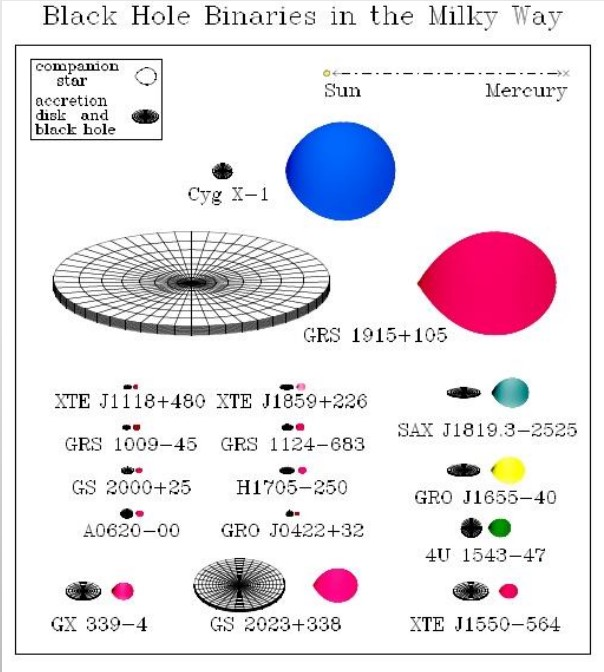
\includegraphics[width=0.7\linewidth]{13_compact}
	\caption{Примеры и масштабы рентгеновских источников}
	\label{fig:13_compact}
\end{figure}

Как мы можем утверждать, что внутри аккреционного диска расположена именно черная дыра?

\begin{enumerate}
	\item В отличии от нейтронных звезд, у которой есть поверхность и магнитное поле, а также она вращается, мы бы наблюдали "пульсации" излучения, связанные с этим вращением нашего диполя-нейтронной звезды. Однако пульсации могут не быть и у нейтронных звезд со слабым магнитным полем(про это задача в дз5, задача 1).
	\item Особенности излучения ЧД. Например, в отличии от нейтронной звезды, у которой вещество на радиусе остановки образует некий пограничный слой, растекаясь по поверхности и это можно детектировать в спектре мощности, у черной дыры внутренняя граница аккреционного диска определяется самой внутренней устойчивой круговой орбитой и нет схожих проявлений в спектре.
	\item Оценкой массы можно исключить из рассмотрения нейтронные звезды, потому что их масса не может превышать ~3 масс Солнца.
\end{enumerate}

Некоторые из таких двойных систем являются \textbf{Рентгеновскими новыми}, в которых аккреция является нестационарной, и выброс энергии идет вспышками. Они дают оценку получше, потому что есть две фазы: когда видно в основном яркий аккреционный диск(вспышка), и когда видно тусклый красный карлик(спокойное состояние; из рисунка \ref{fig:13_compact}, именно КК обычно входят в состав такой системы), поэтому оценка на массу получается лучше.

Однако и нейтронные звезды могут быть такими транзиентными(непостоянными) источниками, но отличить их можно по минимальной светимости в этой спокойной фазе. В этой фазе всё равно есть небольшое перетекание массы с КК, но из-за отсутствие поверхности у черной дыры она не эффективно перерабатывает это небольшое кол-во материала в энергию, в отличии от нейтронной звезды, которая своей магнитосферой размазывает вещество по поверхности и тем самым не может светить тусклее черной дыры.

К тому же, у систем с нейтронной звездой имеется явление 'Рентгеновского барстера' - если кратко, это накапливание вещества у поверхности звезды, после которого идет вспышка(из-за термоядерной реакции на поверхности) в рентгеновском диапазоне. У некоторых систем такое не наблюдается, и простое объяснение - там нет поверхности, где бы накапливалось вещество, то есть мы имеем дело с черной дырой.

\begin{figure}[H]
	\centering
	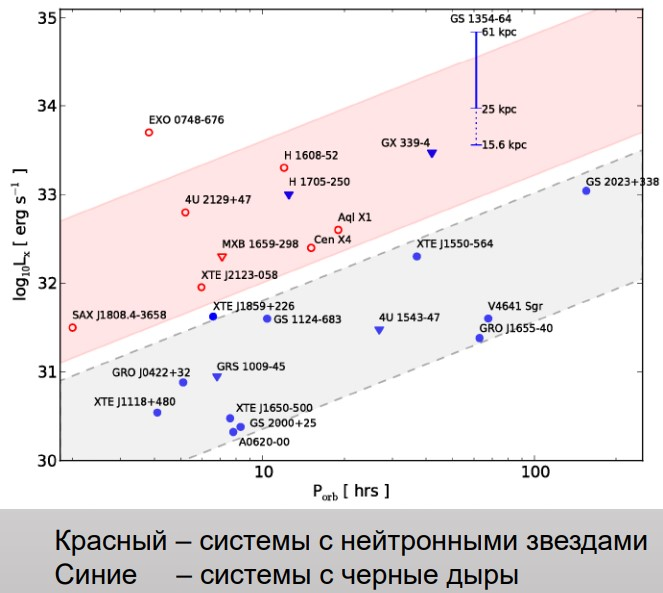
\includegraphics[width=0.7\linewidth]{13_xray_new}
	\caption{Светимость систем с НЗ и ЧД}
	\label{fig:13_xray_new}
\end{figure}

\subsection{Двойная система из черных дыр}

Интересным случаем является двойная система двух черных дыр, а именно явление \textbf{слияния черных дыр}, детектировать которое мы можем по гравитационным волнам, характерная длина волн которых порядка этой системы дыр, то есть величины порядка 100 км и более).

	
	\newpage
	
	\section{Сверхмассивные черные дыры, методы определения их масс.}
Сверхмассивные чёрные дыры наблюдаются в центрах галактик, хотя находятся не тодбко там.

Так как квазары -- очень далекие объекты относительно небольшого размера (доли парсека), для объяснения их аномально высоких светимостей была высказана гипотеза об аккреции вещества сверхмассивными черными дырами(десятки млн. масс Солнца).

\subsection{Пример: сверхмассивная чёрная дыра M31(туманность Андромеды)}

Сверхмассивные чёрные дыры встречаются в центральных частях многих галактик. В центральной части Галактики м31 (Туманность Андромеды) есть сверхмассивная черная дыра массой около $10^8 M_{sun}$ и светимостью $L \sim 10^{36} \text{ эрг/с}$. Значение массы очень приблизительное, так как на больших расстояниях измерить точные траектории движения отдельных звёзд невозможно (расстояние до центра туманности Андромеды в 100 раз больше, чем до центра нашей галактики).

Сейчас чёрная дыра ''спит'', имея светимость значительно менььше эддингтоновской.

\subsection{Методы определения масс}

Всегда можно дать оценку сверху на массу черной дыры, исходя из того, что светимость не превосходит эддингтоновскую, но эта оценка слишком грубая.

\paragraph{Мазеры} Самый точный метод измерения массы очень далекой черной дыры.

Идея заключается в том, чтобы найти объект, вращающийся около черной дыры и точно его измерить: в нашей галактике это звёзды, в других -- мазерные источники, испускающие излучение строго а одной частоте, а значит, по изменению этой частоты можно определить скорость движения мазера. Если он находится близко к чёрной дыре ($<$ 1 пк), его движение будет определяться массой черной дыры, а значит этот метод будет давать точный результат.
\begin{wrapfigure}{r}{0.4\linewidth}
  \centering
    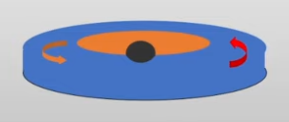
\includegraphics[width=0.7\linewidth]{Pictures/14_disk.png}
  \caption{Движение слоёв газа вокруг черной дыры.}
  \label{fig:14_disk}
 \end{wrapfigure}
\paragraph{Кинематика газа} Метод применим для близких чёрных дыр.


Если нет мазеров, иногда можно пронаблюдать изменение движения газа в диске вокруг чёрной дыры, измерив спектральные характиристики (измерить, с какой скоростью вращаются вокруг чёрной дыры разные части диска). Например, если вещество движется в сторонуь наблюдателя, за счёт эффекта Доплера, оно синеет $\implies$ все сдвигается в синюю часть спектра.

\newpage

\begin{wrapfigure}[11]{l}{0.4\linewidth}
  \centering
    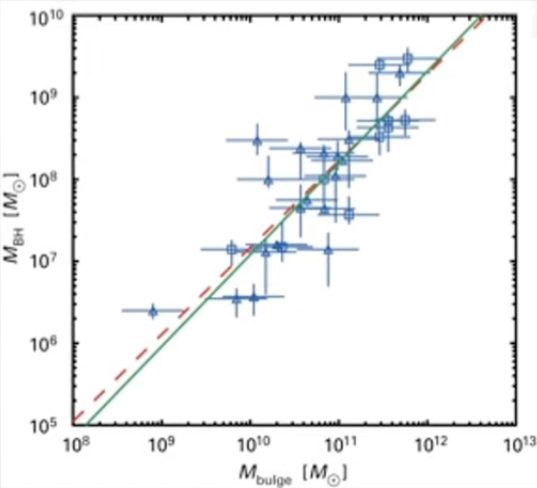
\includegraphics[width=0.7\linewidth]{Pictures/14_kor.png}
  \caption{Корреляция масс}
  \label{fig:14_kor}
 \end{wrapfigure}
\paragraph{Корреляция с масссой балджа}

Балдж (от англ. bulge — «вздутие») — центральный яркий эллипсоидальный компонент спиральных и линзообразных галактик. Размер его колеблется от сотен парсеков до нескольких килопарсеков. Балдж галактики состоит в основном из старых звёзд, движущихся по вытянутым орбитам. Составляет внутреннюю, наиболее плотную часть сферической подсистемы галактики. В центре нередко содержится сверхмассивная чёрная дыра. Её масса коррелирует с балджем галактики как $M_{BH}\sim M_{buldge}^{1.12\pm 0.6}$.


\paragraph{Фанфакты}
\paragraph{Откуда берутся сверхмассивные черные дыры?}

Самый реалистичный сцентарий возникновения -- эволюция звезд первого поколения. Они состояли из чистой водородно - гелиевой смеси, были очень большими и массивными, возникли раньше, чем галактики. Эволюционно они переходили в стадию чёрной дыры, а на стадии появления галактик группы звёзд собирались в скопления и чёрная дыра оседала в центре. Постепенно ее масса росла, а взаимодействие с массивными объектами выкидывало недостаточно массивные дыры из галактик.

Альтернативная теория необходима в силу того что наблюдаются чёрные дыры слишком массивные для такого вида образования (исходя из предела на светимость). То есть начальная масса чёрной дыры должна быть значительно больше 100-200 масс Солнца, как это было бы в сценарии первых звезд. Поэтому существует теория появления сверхмассивных чёрных дыр путем коллапса больших облаков газа в единый объект, которы образует что-то вроде свермассивной звезды, которая с течением времени схлопывается в огромную черную дыру.

\paragraph{Гравитационное поле}

Еще одна интересная форма активности черных дыр связана с их мощным грави-тационным полем. При приближении объекта к черной дыре, возникают приливныесилы, которые стремятся его разорвать. Сверхмассивные черные дыры могут раз-рывать не слишком компактные звезды, они легко разрывают красные гиганты. Вцентре довольно сложная структура сингулярности.
	
	\newpage
	
	\section{Наша Галактика: строение и основные параметры.}
\subsection{Основные сведения}
Галактика (Млечный Путь) -- спиральная галактика с перемычкой, в которой находится солнечная система. Млечный Путь вместе с галактикой Андромеды (М31), галактикой Треугольника (М33) и более чем 40 карликовыми галактиками-спутниками — своими и Андромеды — образуют Местную группу галактик которая входит в Местное сверхскопление (Сверхскопление Девы). 
\begin{figure}[H]
    \centering
    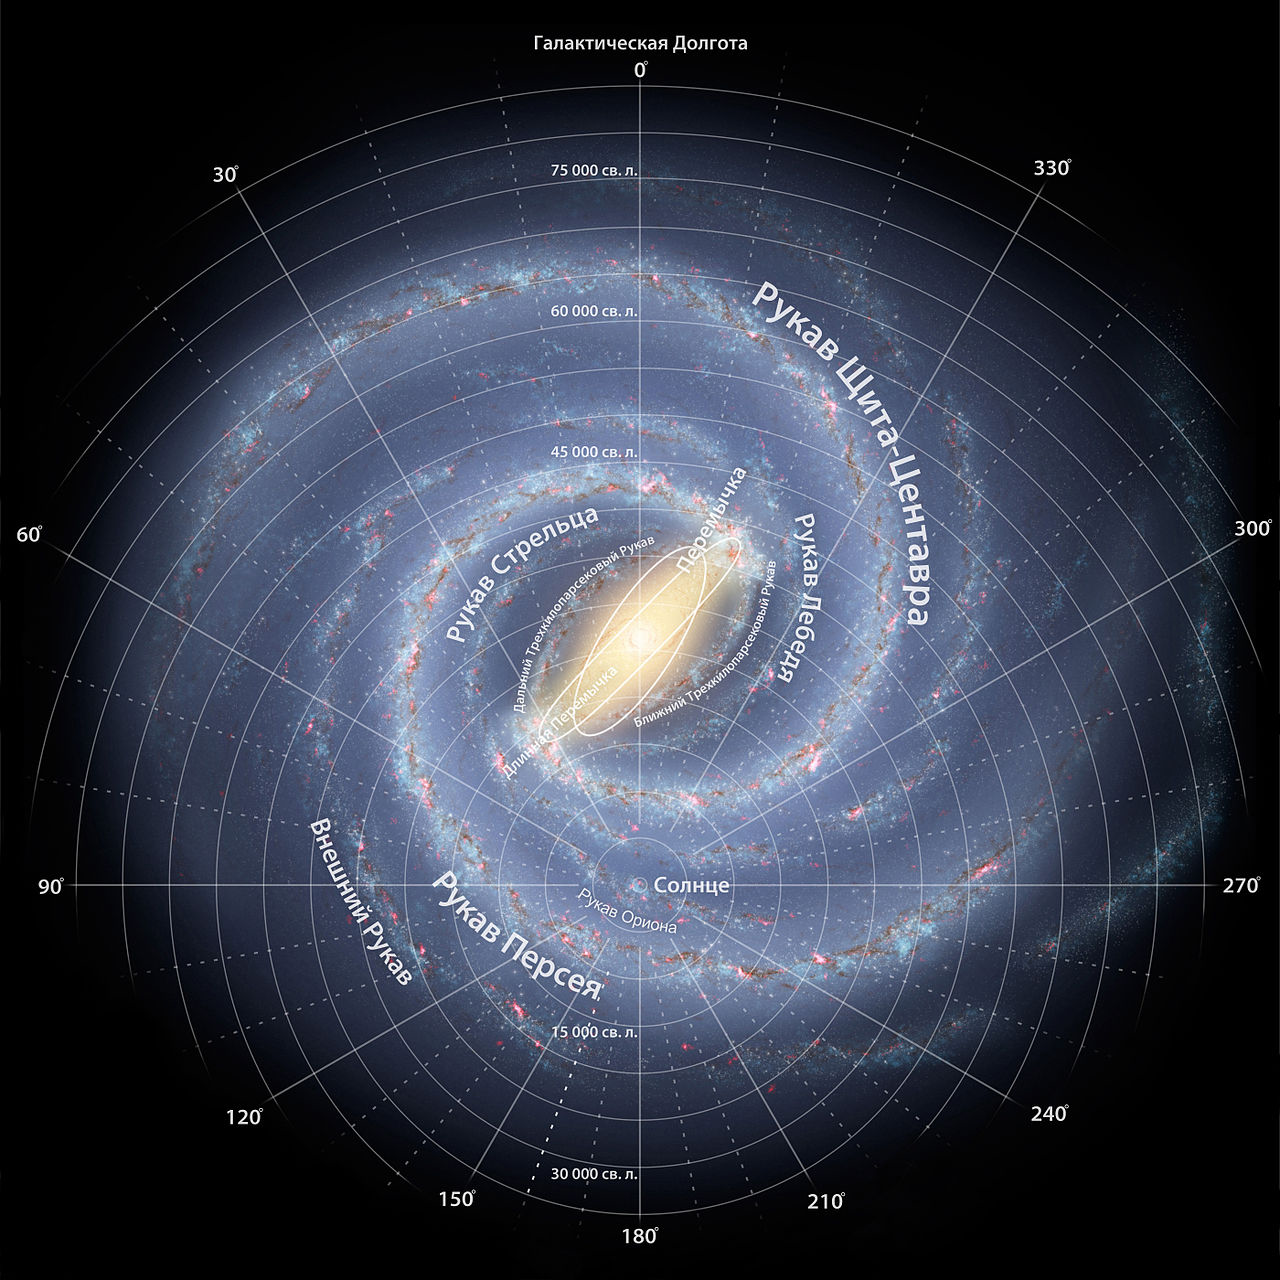
\includegraphics[scale=0.3]{15_galaxy.png}
    \caption{Рукава Млечного Пути.}
    \label{fig:galaxy_1}
\end{figure}
\subsection{Строение и параметры}
Млечный Путь — спиральная галактика с перемычкой («баром») из ярких звёзд, выходящей из центра и пересекающей галактику посередине. Спиральные ветви галактики начинаются на концах перемычки, тогда как в обычных спиральных галактиках они выходят непосредственно из ядра. Основные ветви (рукава) приведены на рисунке~\ref{fig:galaxy_1}.  
\begin{figure}[H]
    \centering
    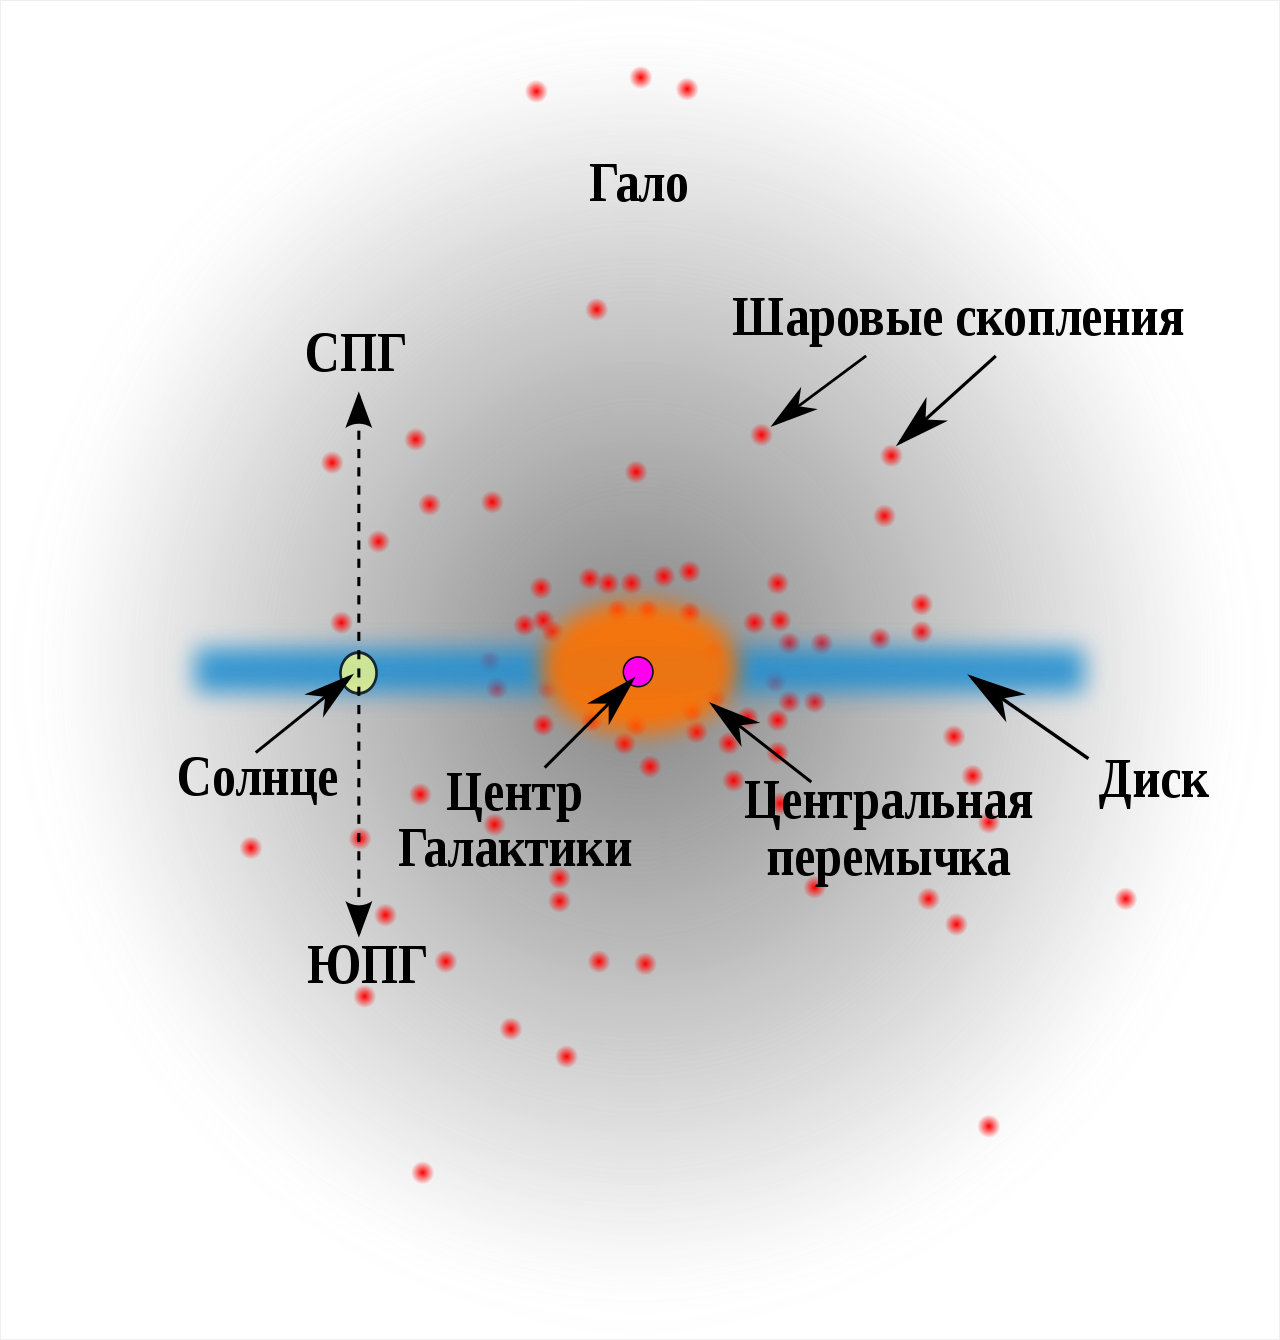
\includegraphics[scale=0.2]{15_galaxy_structure.png}
    \caption{Схематическое изображение структуры Галактики. ЮПГ и СПГ -- южный и северный полюса галактики.}
    \label{fig:galay_2}
\end{figure}
\subsubsection{Размеры}
Диаметр Галактики составляет около 30 тыс. парсек (порядка 100 000 световых лет, 1 квинтиллион километров), при оценочной средней толщине порядка 1000 световых лет.
\subsubsection{Количество звёзд}
Галактика содержит, по современной оценке, от 200 до 400 миллиардов звёзд. Их основная масса расположена в форме плоского диска.
\subsubsection{Масса}
Б\'{о}льшая часть массы Галактики содержится не в звёздах и межзвёздном газе, а в несветящемся гало из тёмной материи, поэтому точное определение массы Млечного Пути весьма затруднено.

В 2019 году, объединив новые данные миссий «Gaia» и «Hubble», астрономы определили, что масса Млечного Пути, в радиусе 129 000 световых лет от центра Галактики, составляет около $1.5\cdot10^{12}$ масс Солнца.
\subsubsection{Диск}
По оценкам учёных, галактический диск, выдающийся в разные стороны в районе галактического центра, имеет диаметр около 100 000 световых лет. По сравнению с гало, диск вращается заметно быстрее. Скорость его вращения неодинакова на различных расстояниях от центра. Она стремительно возрастает от нуля в центре до 200—240 км/с на расстоянии 2 тыс. световых лет от него, затем несколько уменьшается, снова возрастает примерно до того же значения и далее остаётся почти постоянной. Изучение особенностей вращения диска позволило оценить его массу, оказалось, что она в 150 млрд раз больше массы Солнца.

Вблизи плоскости диска концентрируются молодые звёзды и звёздные скопления, возраст которых не превышает нескольких миллиардов лет. Они образуют так называемую плоскую составляющую. Среди них очень много ярких и горячих звёзд. Газ в диске Галактики также сосредоточен в основном вблизи его плоскости. Он распределён неравномерно, образуя многочисленные газовые облака — от гигантских неоднородных по структуре облаков, протяжённостью свыше нескольких тысяч световых лет, к небольшим облакам размерами не более парсека.
\subsubsection{Центр Галактики}
В средней части Галактики находится утолщение, которое называется балджем, составляющее около 8300 парсек (27 000 световых лет) в поперечнике. Центр ядра Галактики находится в направлении Созвездия Стрельца ($\alpha = 265^{\circ}$, $\delta = - 29^{\circ}$). Расстояние от Солнца до центра Галактики 8500 парсек ($2.62\cdot10^{17}$ км, или 27 700 световых лет). В центре Галактики, по всей видимости, располагается сверхмассивная чёрная дыра (Стрелец $A^{*}$) (около 4,3 миллиона масс Солнца) вокруг которой, предположительно, вращается чёрная дыра средней массы от $1000M_{\Sun}$ до $10 000M_{\Sun}$ и периодом обращения около 100 лет и несколько тысяч сравнительно небольших. Их совместное гравитационное действие на соседние звёзды заставляет последние двигаться по необычным траекториям.

Для центральных участков Галактики характерна сильная концентрация звёзд: в каждом кубическом парсеке вблизи центра их содержатся многие тысячи. Расстояния между звёздами в десятки и сотни раз меньше, чем в окрестностях Солнца. Как и в большинстве других галактик, распределение массы в Млечном Пути такое, что орбитальная скорость большинства звёзд Галактики не зависит в значительной степени от их расстояния до центра. Далее от центральной перемычки к внешнему кругу обычная скорость обращения звёзд составляет 210—240 км/с. Такое распределение скорости, не наблюдаемое в Солнечной системе, где различные орбиты имеют существенно различные скорости обращения, является одним из указаний на существование тёмной материи.

Считается, что длина галактической перемычки составляет около 27 000 световых лет. Эта перемычка проходит через центр галактики под углом $44 \pm 10$ градусов к линии между нашим Солнцем и центром галактики. Она состоит преимущественно из красных звёзд, которые считаются очень старыми. Перемычка окружена кольцом, называемым «Кольцом в пять килопарсек». Это кольцо содержит большую часть молекулярного водорода Галактики и является активным регионом звездообразования в нашей Галактике. Если вести наблюдение из галактики Андромеды, то галактическая перемычка Млечного Пути была бы яркой его частью.
\subsubsection{}
Галактическое гало имеет сферическую форму, выходящую за пределы галактики на 5—10 тысяч световых лет, и температуру около $5\cdot105$ K. Галактический диск окружён сфероидным гало, состоящим из старых звёзд и шаровых скоплений, 90 \% которых находится на расстоянии менее 100 000 световых лет от центра галактики. Однако в последнее время было найдено несколько шаровых скоплений, таких как Pal 4 и AM 1, находящихся на расстоянии более чем 200 000 световых лет от центра галактики. Центр симметрии гало Млечного Пути совпадает с центром галактического диска. Состоит гало в основном из очень старых, неярких маломассивных звёзд. Они встречаются как поодиночке, так и в виде шаровых скоплений, которые могут содержать до миллиона звёзд. Возраст населения сферической составляющей Галактики превышает 12 млрд лет, его обычно считают возрастом самой Галактики.

В то время как галактический диск содержит газ и пыль, что затрудняет прохождение видимого света, сфероидная компонента таких составляющих не содержит. Активное звездообразование происходит в диске (особенно в спиральных рукавах, являющихся зонами повышенной плотности). В гало звездообразование завершилось. Рассеянные скопления также встречаются преимущественно в диске. Считается, что основную массу нашей галактики составляет тёмная материя, которая формирует гало тёмной материи массой примерно 600—3000 миллиардов масс Солнца. Гало тёмной материи сконцентрировано в направлении центра галактики.

Звёзды и звёздные скопления гало движутся вокруг центра Галактики по очень вытянутым орбитам. Так как вращение отдельных звёзд происходит несколько беспорядочно (то есть скорости соседних звёзд могут иметь любые направления), гало в целом вращается очень медленно.
\subsection{Положение Солнца в Галактике}
Согласно последним научным оценкам, расстояние от Солнца до галактического центра составляет $27 000 \pm 1 400$ световых лет, в то время как, согласно предварительным оценкам, наша звезда должна находиться на расстоянии около 35 000 световых лет от перемычки. Это означает, что Солнце расположено ближе к краю диска, чем к его центру. Вместе с другими звёздами Солнце вращается вокруг центра Галактики со скоростью 220—240 км/с, делая один оборот примерно за 200 млн лет. Таким образом, за всё время существования Земля облетела вокруг центра Галактики не более 30 раз.

	
	\newpage
	
	\section{Типы галактик, эволюция галактик}

\subsection{Типы галактик}

Галактики согласно классификации Хаббла делятся на эллиптические (E), спиральные (S) и неправильные (Irr). Примеры красивых картинок можно найти на рисунке \ref{fig:16_galaxy_types}.

\begin{figure}[H]
	\centering
	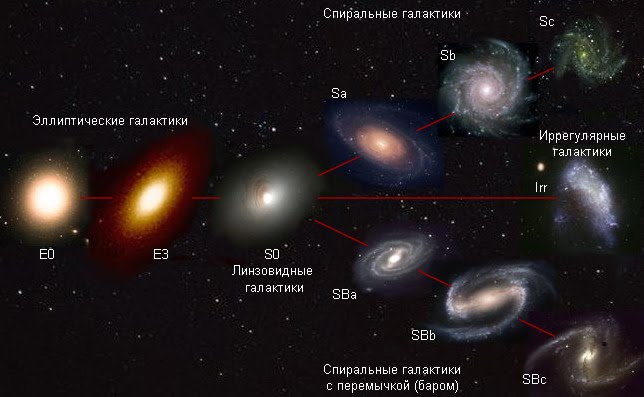
\includegraphics[width=0.9\linewidth]{16_galaxy_types}
	\caption{Типы галактик: эллиптические (E), спиральные (S) и неправильные (Irr)}
	\label{fig:16_galaxy_types}
\end{figure}

\subsubsection{Эллиптические галактики}

Эллиптические галактики имеют эллиптическую форму и характеризуются равномерной яркостью, которая постепенно убывает от края к центру.

Форма галактик данного типа варьируется от практически совершенно круглой, до сплюснутого эллипса. Соответственно для обозначения степени сплюснутости галактики к букве Е прибавляется число n, определяемое по формуле: $n = 10 (a - b) / a$, где $ a$, $b$, - это соответственно большая и малая полуоси галактики. Таким образом, эллиптическая галактика круглой формы будет отнесена к типу Е0, а сплюснутая может быть классифицирована, например, как $E3$.

\subsubsection{Спиральные галактики}

В спиральных галактиках ядро представляет собой наиболее яркую область, обладающую признаками эллиптических галактик. Наличие в спиральной галактике перемычки (бара) позволяет разделить их на два основных типа. К первому относятся нормальные спиральные галактики, обозначаемые буквой (S). Ко второму типу относятся так называемые пересеченные галактики, обозначаемые (SB). Для более точной характеристики той или иной галактики, деления их всего на 2 типа недостаточно. Поэтому Хаббл классифицировал спиральные галактики по следующим трем критериям:

\begin{enumerate}
	\item Относительной величине ядра, по сравнению с размерами всей галактики;
	
	\item По тому, насколько сильно или слабо закручены спиральные ветви;
	
	\item Фрагментарности спиральных ветвей.
\end{enumerate}

К типу Sa или (SBa) относятся галактики с очень обширной ядерной областью и сильно закрученными спиральными ветвями - непрерывными и гладкими, а не фрагментарными.

Галактики типа Sb и SBb имеют относительно небольшую ядерную область, и не очень сильно закрученные спиральные ветви, которые разрешаются на отдельные яркие фрагменты. Галактики типа Sc и SBc характеризуются сильно фрагментарными обрывочными спиральными рукавами. У галактик SBc даже бар разделяется на отдельные фрагменты.

Кроме того, отдельно выделен тип галактик, промежуточный, между спиралями и эллиптическими системами, - галактики типа SO. У них чрезвычайно толстый диск, мощный балдж и не видно спиральных ветвей. Кстати, обозначив этот тип галактик буквой S, несмотря на отсутствие спиралей, Хаббл тем самым подчеркнул, что главным в различии спиральных и эллиптических систем является звездный диск.

\subsection{Эволюция галактик}
Единой теории образования и эволюции галактик нет. Возможные теории образования галактик:
\begin{itemize}
	\item \textbf{Иерархическая теория} предполагает, что уже после возникновения первых звёзд во Вселенной начался процесс гравитационного объединения звёзд в скопления и далее в галактики. 
	
	Недостаток: современные наблюдения показывают, что на \(z \approx 10\) (спустя 400 млн после Большого взрыва) уже существовали сформировавшиеся галактики, но между возникновением первых звезд и вышеуказанным периодом прошло слишком мало времени, так что галактики сформироваться не успели бы.
	
	\item \textbf{Инфляционная теория}. Во время расширения вселенной со сверхсветовой скоростью (инфляционного расширения) происходили квантовые флуктуации. Квантовые флуктуации расширялись вместе со всей вселенной, причем до порядков, в \(10^{10^{12}}\) раз превышающих исходный. Те из них, которые существовали в момент прекращения инфляции, остались <<раздутыми>> и оказались первыми тяготеющими неоднородностями во Вселенной. Получается, что у материи было порядка 400 млн лет на гравитационное сжатие вокруг этих неоднородностей и образование газовых туманностей. А далее начался процесс возникновения звёзд и превращения туманностей в галактики.
\end{itemize}

В процессе эволюции галактики могут сливаться друг с другом. Результатом слияния галактик, как правило, оказываются эллиптические галактики. В пользу этого говорит тот факт, что звезды в эллиптических галактиках находятся на орбитах, случайно ориентированных внутри галактик.

Прекращение процесса звездообразования в галактиках называется <<тушением галактик>>. Звезды образуются из холодного газа, поэтому галактика гаснет, когда в ней больше нет холодного газа. Однако считается, что тушение происходит относительно быстро (в течение 1 миллиарда лет), что намного меньше времени, которое потребуется галактике, чтобы просто израсходовать свой резервуар холодного газа. Модели эволюции галактик объясняют это гипотезой о других физических механизмах, которые устраняют или перекрывают подачу холодного газа в галактику. Эти механизмы можно в общих чертах разделить на две категории:

\begin{itemize}
	\item Механизмы \textbf{превентивной} обратной связи, которые не позволяют холодному газу проникать в галактику или не дают ему образовывать звезды. Стройной физической концепции нет.
	
	\item Механизмы \textbf{выталкивающей} обратной связи, которые удаляют газ так, чтобы он не мог образовывать звезды. Один из механизмов выброса  вызван сверхмассивными черными дырами, обнаруженными в центрах галактик. Моделирование показало, что газ, аккрецирующий на сверхмассивных черных дырах в центрах галактик, производит струи высокой энергии; высвобожденная энергия может вытеснить достаточно холодного газа, чтобы погасить звездообразование.
\end{itemize}
	
	\newpage
	
	\section{Тёмное вещество. Ключевые наблюдательные свидетельства.}
\begin{figure}[H]
    \centering
    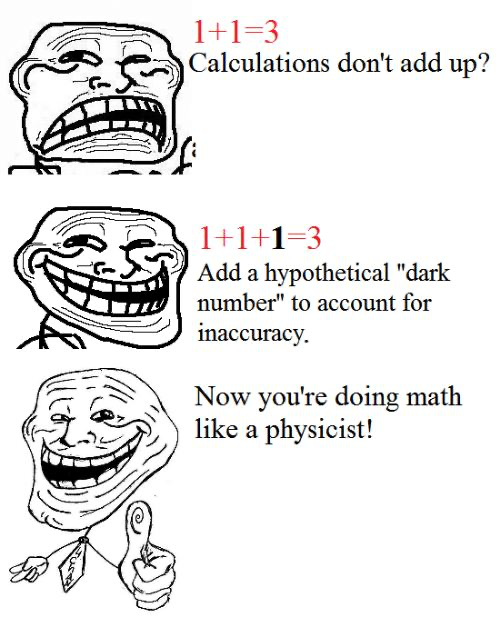
\includegraphics[scale=0.5]{17_memes.png}
    \caption{Билет вкратце.}
    \label{fig:memes}
\end{figure}
\subsection{Тёмное вещество}
Тёмная материя в астрономии и космологии, а также в теоретической физике — гипотетическая форма материи, не участвующая в электромагнитном взаимодействии и поэтому недоступная прямому наблюдению. Составляет порядка четверти массы-энергии Вселенной и проявляется только в гравитационном взаимодействии. Понятие тёмной материи введено для теоретического объяснения проблемы скрытой массы в эффектах аномально высокой скорости вращения внешних областей галактик и гравитационного линзирования (в них задействовано вещество, масса которого намного превышает массу обычной видимой материи); среди прочих предложенных оно наиболее удовлетворительно.
\subsection{Ключевые наблюдательные свидетельства.}
\subsubsection{Вращение звёзд в галактиках.}
\begin{figure}[H]
    \centering
    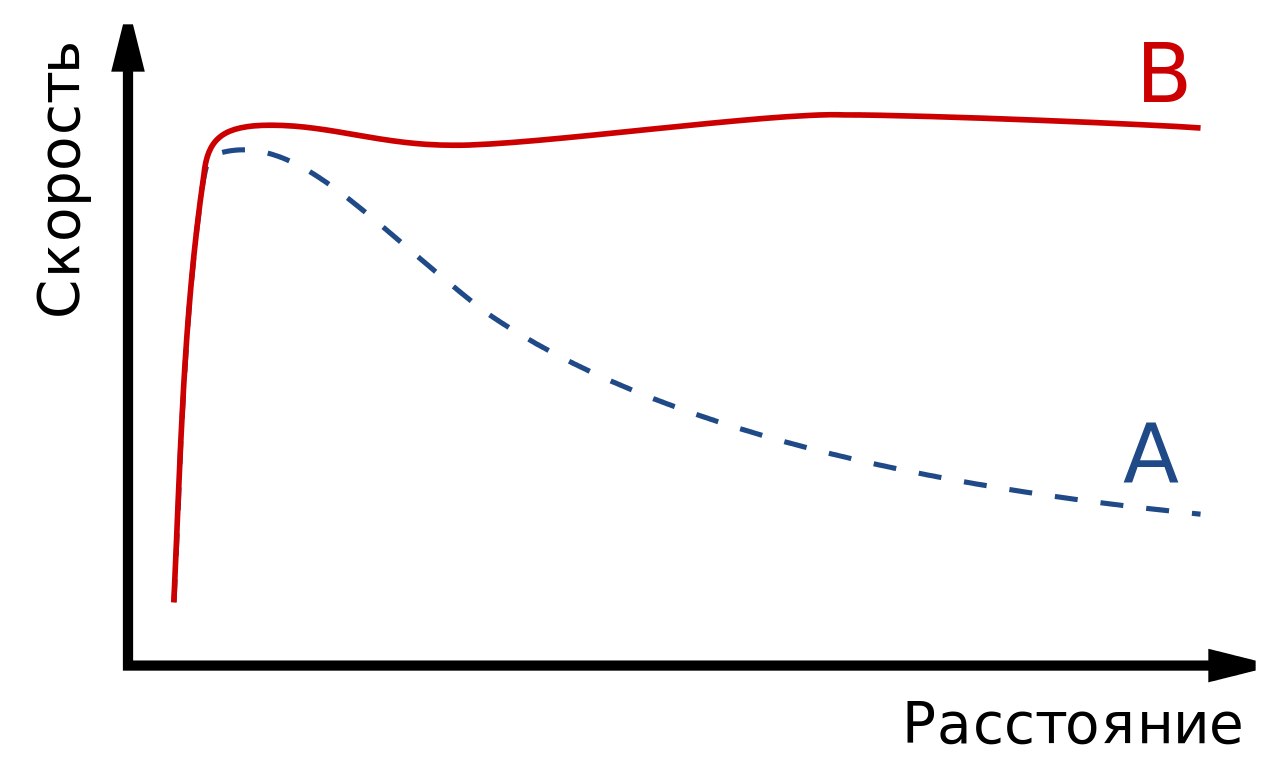
\includegraphics[scale=0.2]{17_curve.png}
    \caption{Кривая вращения галактики: (A) ожидаемая; (B) реальная.}
    \label{fig:galaxy_curve}
\end{figure}
Кривые вращения галактик, демонстрирующие отсутствие убывания скорости вращения на периферии звёздных дисков. Наиболее простым объяснением этого эффекта является наличие у галактик массивных невидимых гало, дающих большой вклад в их массы.
\subsubsection{Движение галактик-спутников и шаровых скоплений возле массивных галактик.}
Мелкие галактики-спутники движутся вокруг крупных, подчиняясь тем же законам, что и звёзды на периферии обычных галактик, таким образом являясь пробными телами такого же рода, но на большем масштабе, что позволяет делать выводы о распределении гравитационного потенциала таких массивных галактик. Анализ данных для нашей и других галактик подтвердил, что общая масса каждой галактики в несколько раз превышает суммарную массу её звёзд.
\subsubsection{Большие системы}
Динамика систем галактик от двойных галактик до галактических скоплений. Анализ лучевых скоростей их членов даёт характерный разброс скоростей галактик, что позволяет оценить полные массы этих систем. Таким образом выявлено, что тёмная материя присутствует на всех уровнях галактической иерархии, причём её доля растёт с увеличением масштаба: в двойных системах она превышает вклад видимой материи в несколько раз, а в скоплениях галактик (состоящих из сотен и тысяч объектов) — в десятки или сотни раз.
\subsubsection{Распределение горячего газа в эллиптических галактиках}
Рентгеновское излучение горячего газа в гигантских эллиптических галактиках и их скоплениях, зарегистрированное такими орбитальными обсерваториями как «Эйнштейн», «ROSAT», «XMM-Newton» и «Чандра». С помощью рентгеновских телескопов определяется распределение поверхностной яркости (в рентгеновском диапазоне) и температуры таких объектов в двумерной проекции, на основании этих характеристик строится радиальное распределение плотности и температуры газа, что даёт возможность получить массовый профиль галактики или скопления, исходя из условия гидростатического равновесия. Это важное преимущество такого метода, поскольку иные дают лишь значение полной массы объекта. Масса одних лишь звёзд и газа, согласно расчётам, недостаточна для удержания входящего в галактики и скопления горячего газа, если не учесть тёмную материю. Такой горячий газ составляет лишь порядка 15 \% всей массы скоплений, светящаяся видимая материя — ещё меньше, всего 5 \%, и оставшиеся 80 \% представляют собой тёмную материю. При этом радиальное распределение газа (в зависимости от расстояния до центра объекта) примерно повторяет гипотетическое распределение тёмной материи — профиль Наварро — Френка — Уайта.
\subsubsection{Гравитационное линзирование}
Гравитационное линзирование — отклонение света удалённых объектов гравитационным полем находящихся на его пути массивных скоплений, ввиду чего изображения более удалённых галактик, проецирующихся на некое наблюдаемое скопление, оказываются искажёнными (слабое гравитационное линзирование) или даже расщепляются на несколько «копий» (сильное гравитационное линзирование). По характеру этих искажений становится возможным восстановить распределение и величину массы внутри скопления, в том числе скрытой.

	
	\newpage
	
	
\section{ Закон Хаббла. Расстояния в космологии.}

Вселенная расширяется. Точного описания этого эффекта нет, но существуют различные модели(типа \href{https://en.wikipedia.org/wiki/Lambda-CDM_model}{$\Lambda$CDM}, о которой также пойдет речь) описания этого.

В данном билете рассказывается о сути закона Хаббла, о вышеупомянутой модели, о различных расстояниях, использумых при описании(потому что в расширяющейся вселенной может быть удобно говорить о разных расстояниях).

\subsection{Расстояния в космологии}

Если представить себе, что всеселнная не расширяется, а объекты не имеют пекулярных скоростей(то есть абсолютно всё покоится), то именно в такой системе мы можем говорить о \textbf{сопутствующих расстояниях(comoving distance)} - расстояниях в системе отсчета, когда мы зафиксировали все галактики в какой-то момент времени(это важно - фиксируют его для текущего времени). Обозначать его я буду буквой $\chi$.

\textbf{Собственное расстояние(proper distance)} определяется через масштабный фактор a:

\begin{equation}
d = a \cdot \chi
\label{eq:18_proper}
\end{equation}

Наблюдая свет, приходящей от галактики, мы можем измерять \textbf{красное смещение} z, смотря на особые спектральные линии(например линия 21 см или линия HI). Красным оно называется, потому что длина волны увеличивается, тем самым смещая спектр в сторону длинноволнового. Определение и связь смещения с масштабным фактором показаны на рисунке \ref{fig:18_redshift}.

\begin{figure}[H]
	\centering
	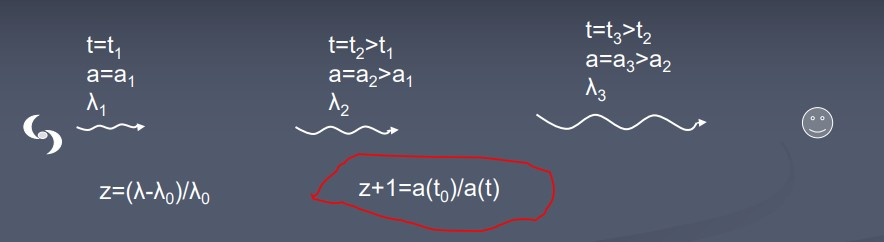
\includegraphics[width=0.7\linewidth]{18_redshift}
	\caption{Красное смещение}
	\label{fig:18_redshift}
\end{figure}

Есть так называемое \textbf{фотометрическое расстояние} - оно определяется из формулы для потока:

\begin{equation}
f = \frac{L}{4 \pi d_{ph}^2}
\label{eq:18_photometric}
\end{equation}

Таким образом, оно просто связывается с собственным расстоянием, умножая его на (1+z), потому что именно во столько(из определения) уменьшается энергия фотонов:

\begin{equation}
d_{ph} = \frac{a(t_0)}{a(t_{em})} \cdot d = \frac{a^2(t_0)}{a(t_{em})} \chi
\label{eq:18_photo_proper}
\end{equation}

Существует еще одно важное расстояние - \textbf{Угловое(угломерное) расстояние}. Зная размер галактики s, зная угол под которым мы видим галактику, мы можем использовать классическую формулу для определения расстояния:

\begin{equation}
d_{\theta} = \frac{s}{tg(\alpha)}
\label{eq:18_angular}
\end{equation}

По предположению, вселенная плоская(в том смысле, что у нее нет кривизны), и потому угол между фотонами сохраняется во времени. Однако галактика могла испустить фотон, который мы детектируем, в разные моменты вселенной(так как вселенная эволюционирует, меняется количественное соотношение типов вещества, скорость расширения не остаётся постоянной), поэтому красное смещение не однозначно показывает это расстояние. Из рисунка \ref{fig:18_angular}(слайд с лекции), для галактик с одинаковым s в разные моменты времени z может быть разным(но собственное расстояние будет одинаковым на момент испускания):

\begin{figure}[H]
	\centering
	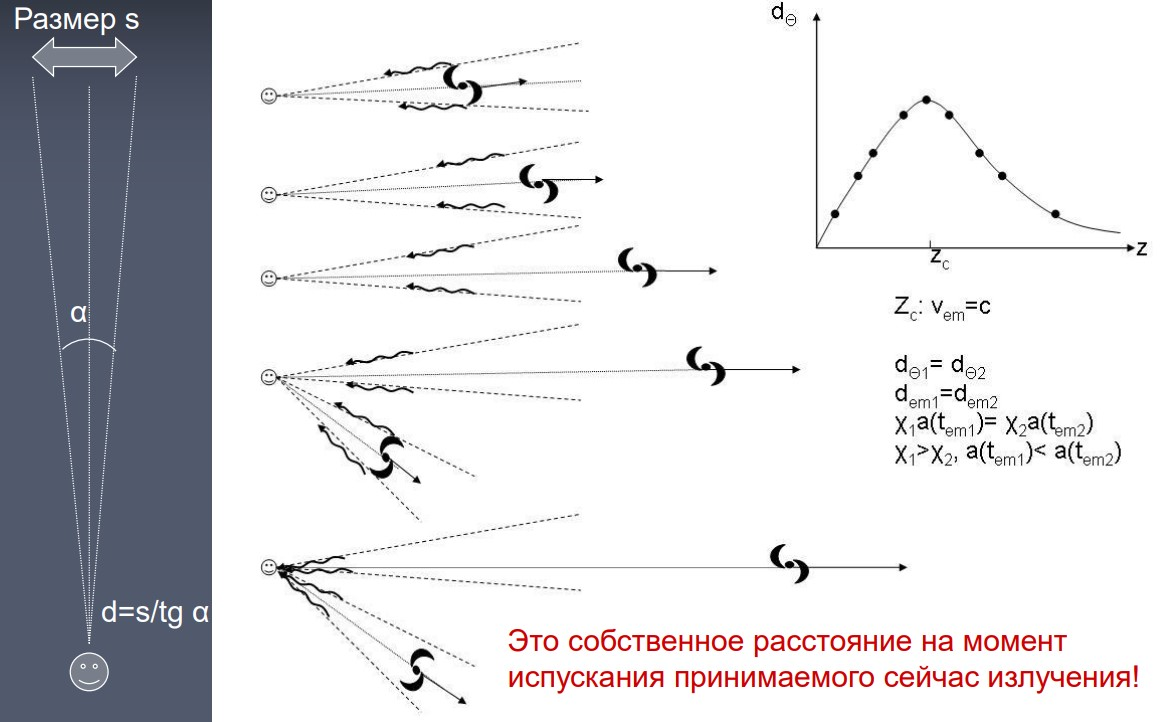
\includegraphics[width=0.7\linewidth]{18_angular}
	\caption{Угловое(углометрическое) расстояние}
	\label{fig:18_angular}
\end{figure}

Мы ввели все основные расстояния, которые и будем связывать друг с другом, но есть еще одно - время путешествия(жизни) фотона. Оно лежит где-то между собственным расстоянием в момент испускания фотона, и собственным расстоянием в настоящий момент.

\begin{equation}
d_l = c \cdot \Delta t
\label{eq:18_lifetime}
\end{equation}

Связь всех этих величин такая($d_{pm}$ - собственное расстояние в настоящий момент, $t_{em}$ - момент испускания фотона):

\begin{equation}
d_{\theta} = a(t_{em}) \chi = \frac{d_{pm}}{1+z} = \frac{d_{ph}}{(1+z)^2}
\label{eq:18_link}
\end{equation}

При этом расстояние $d_{pm} = d$ можно вычислить через постоянную Хаббла(о ней следующий пункт), красное смещение и скорость света:

\begin{equation}
d = \frac{c}{(1-\alpha)H_0} [(1 + z)^{1-\alpha} - 1]
\label{eq:18_distance_h}
\end{equation}

\subsection{Закон Хаббла}

Закон Хаббла в классическом определении - связь скорости удаления галактик в зависимости от собственного расстояния между ними. $H_0$ - коэффициент пропорциональности, называемый постоянной Хаббла(которая на самом деле не постоянна, но берется значение в текущий момент времени).

\begin{equation}
v = H_0 r
\label{eq:18_classic_hubble}
\end{equation}

Сформулировать закон можно также и через масштабный фактор:

\begin{equation}
v = \dot{d}, d = a(t) \chi; \implies v = H d,  H = \frac{\dot{a}(t)}{a(t)}
\label{eq:18_hubble_law}
\end{equation}

Это был вывод в предположении, что галактики не имеют пекулярных скоростей(иначе сама $\chi$ не будет const).

Опуская то, откуда мы это знаем(нам дал \href{https://en.wikipedia.org/wiki/Friedmann_equations}{Бог}), масштабный фактор имеет степенную зависимость от времени, и степень разная для разных типов среды, доминирующих во вселенной:

\begin{equation}
a(t) \sim t^{\frac{1}{\alpha}}, \text{Пыль(материя), $\alpha=1.5$; Излучение, $\alpha=2$; Косм.пост.(темная энергия), $\alpha=0$}
\label{eq:18_scale_factor}
\end{equation}

Тогда из \ref{eq:18_scale_factor} и \ref{fig:18_redshift} следует:

\begin{equation}
H = H_0 (1 + z)^{\alpha}
\label{eq:18_hubble_z}
\end{equation}

Тогда, мы можем найти выражение для сопутствующего расстояния(а через него - и для всех остальных):

\begin{multline}
\text{Для света, } 0 = ds^2 = c^2dt^2 - a^2(t)dl^2 \implies \chi = \int dl = \bigg\{ \text{хитро меняя $\frac{dt}{a(t)}$} \\ \text{на $\frac{dz}{a(t_0) H(z)}$} \bigg\} = \frac{c}{a(t_0)} \int_{0}^{z} \frac{dz}{H(z)} = \frac{c}{a(t_0)H_0} \frac{1}{1-\alpha}[(1+z)^{1-\alpha} - 1]
\label{eq:18_distances}
\end{multline}

Отсюда легко получить, почему для близких галактик всё 'по Допплеру':

\begin{equation}
z \ll 1, d = \frac{c z}{H_0}, \text{при этом } d \cdot H_0 = v \implies v = c z, v \sim z
\label{eq:18_semidoppler}
\end{equation}

Когда присутствует несколько типов сред, то выражение для H следующее:
%\href{https://en.wikipedia.org/wiki/Lambda-CDM_model}{$\Lambda$CDM}

\begin{equation}
H^2(z) = H_0^2[\Omega_{radiation}(1+z)^{4} + \Omega_{matter}(1+z)^{3} + \Omega_{curvature}(1+z)^{2} + \Omega_{\Lambda}]
\label{eq:18_hubble_const}
\end{equation}

Где каждое слагаемое в скобках отвечает за свой тип среды: 1 - излучение, 2 - материя, 3 - кривизна(о которой речи не было, по предположению плоскости вселенной), 4 - темная энергия(вакуум, космическая постоянная, 'стоимость существования пространства'), а $\Omega$ - относительное содержание типа среды во вселенной(значение от 0 до 1, $\sum \Omega_i = 1$)

В вышеупомянутой \href{https://en.wikipedia.org/wiki/Lambda-CDM_model}{$\Lambda$CDM} модели, в простой реализации оставляют только 2 и 4 слагаемые, кладя соответствующие $\Omega$ равными ~0.3 и ~0.7 соответственно.

	
	\newpage
	
	\section{Эволюция вселенной: основные наблюдательные свидетельства}

Hubble Ultra-Deep Field -— изображение небольшого региона космоса, составленное из данных, полученных космическим телескопом «Хаббл».


\begin{wrapfigure}[20]{r}{0.6\linewidth}
  \centering
    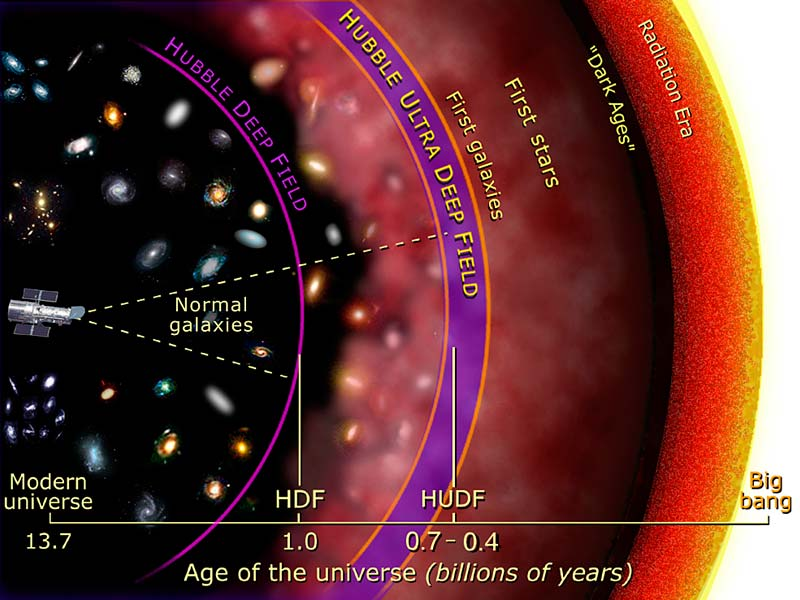
\includegraphics[width=\linewidth]{Pictures/19_hubble.jpg}
  \caption{Диаграмма, отражающая дальность видимости Хаббла}
  \label{fig:19_hubble}
 \end{wrapfigure}
Для обзора была выбрана область неба с низкой плотностью ярких звёзд в ближней зоне, что позволило лучше разглядеть более далёкие и тусклые объекты. Изображение охватывает участок неба диаметром чуть больше 3 угловых минут (1/13 000 000 от всей площади неба), и содержит примерно 10000 галактик.

Типичное расстояние до галактики на глубоком поле Хаббла составляет примено половину возаста Вселенной, следовательно, мы видим далекие галактики молодыми, еще не сформировавшимися.

\subsection{Формирование галактик}

Формы таких дальних галактик довольно причудливые по сравнению с близкими галактиками, так как они взаимодействуют между собой, что стимулирует звездообразования (формируются звёзды из верхнего левого угла диаграммы Герцшпрунга-Рассела \ref{fig:9_diag}).

Это является признаком эволюции вселенной, так как мы можем \textbf{отслеживать темп звездообразования}.
\begin{wrapfigure}[13]{r}{0.3\linewidth}
  \centering
    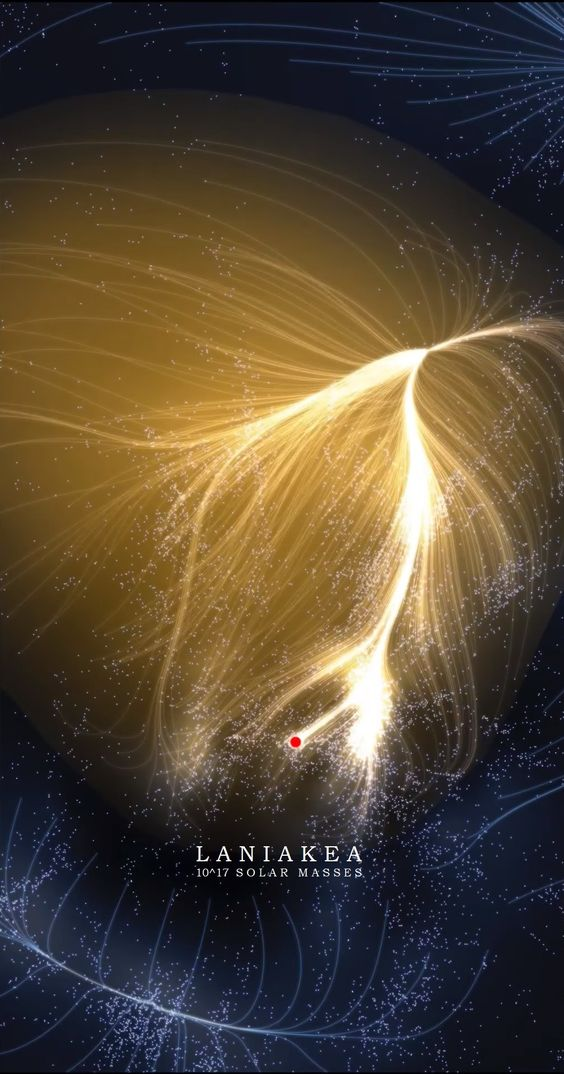
\includegraphics[width=0.7\linewidth]{Pictures/19_lan.jpg}
  \caption{Ланиакея}
  \label{fig:19_lan}
 \end{wrapfigure}
\subsection{Формирование скоплений}

Другим объектом для рассмотрения можно взять скопления галактик на разных расстояниях от нас. Сравнивая разные скопления на разных этапах их формирования, в том числе и эпоху, когда скопления галактик ещё не возникли (1-2 млрд. лет после Большого Взрыва).

\subsection{Ланиакеа}

На расстоянии $\sim 100$ млн. световых лет (что довольно мало) можно довольно точно изучить распределение скоростей галактик (проекций скоростей на луч зрения). Ланиакея (или Ланиакеа) -- это формирующееся сверхскопление галактик, в которую войдут десятки тысяч крупных галактик. Линии -- это треки, а координаты отражают космологические (связанные с расширением вселенной) скорости, которые можно оценить по закону Хаббла. Диаметр Ланиакеи примерно равен 520 миллионам световых лет.

\subsection{Дипольный отталкиватель}
Центр эффективного отталкивания в крупномасштабном течении галактик, находящихся вблизи Млечного Пути, это большие масштабы по сравнению с Ланиакеей: структура, простирающаяся от сверхскопления Шепли до Дипольного отталкивателя, имеет длину почти 1,7 миллиардов световых лет и в 2017 году стала крупнейшим картографированным объектом в наблюдаемой Вселенной. 
\begin{figure}[h]
  \centering
    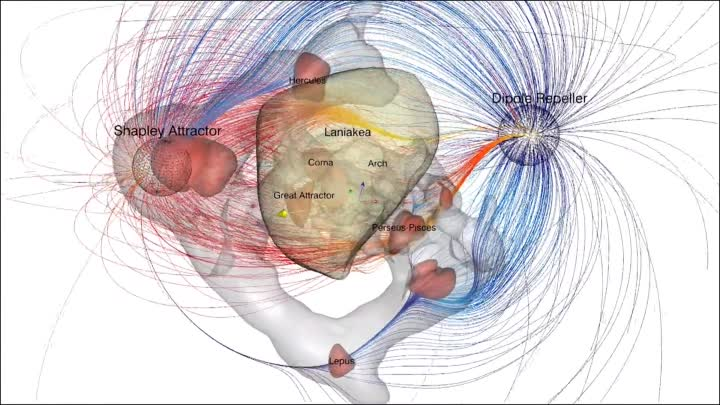
\includegraphics[width=0.7\linewidth]{Pictures/19_dip.jpg}
  \caption{Дипольный отталкиватель и сверхскопление Шепли}
  \label{fig:19_dip}
 \end{figure}
 Этот объект говорит о том, что вселенная эволюционирует, так как мы говорим об изменении морфологии галактик и является важным источником информации.
 
 \subsection{Химическая эволюция}
 
 Есть множевство процессов, приводящих к тому, что легкие элементы превращаются в тяжелые. Изучение областей Вселенной (не только звёзд, но и облаков), но обогащенных тяжелыми элементами, является объектом исследований.
 
 \subsection{Реликтовое излучение}
 
 Можно исследовать эволюцию, измеряя температуру реликтового излучения в разные моменты времени с помощью \textbf{эффекта Сюняева - Зельдовича}.
 После рекомбинации вся Вселенная всегда была заполнена реликтовым излучением, которое имеет спектр, а значит, ему в соответствие можно поставить температуру.
 
 Рассмотрим скопление галактик, где имеется горячий газ, излучающий в рентгеновском диапазоне, а значит, есть электроны с большими скоростями. Фотоны реликтового излучения, имеющие меньшую энергию, будут рассеиваться на этих электронах $\implies$ приобретать энергию. Измеряя реликтовое излучение, мы можем измерить красное смещение (фотоны перебегут на более короткие длины волн). 
 
 По эффекту рассеяния, зная температуру газа в скоплении, мы можем измерить температуру реликтового излучения в разные эпохи.
 
 \begin{figure}
  \centering
    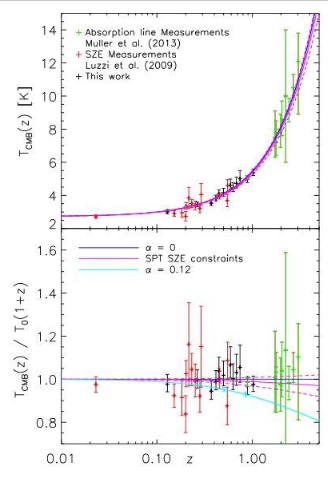
\includegraphics[width=0.5\textwidth]{Pictures/19_imdone.png}
  \caption{Эволюция температуры реликтового излучения}
  \label{fig:19_done}
 \end{figure}

	
	
	
	
	
	
	
	
	
\end{document}